%\documentclass[12pt]{scrreprt}
\documentclass[12pt]{report}

% language may be romanian or english (default is english)
% type may be bachelor or master (default is bachelor)
\usepackage[language=english, type=bachelor]{style}

\usepackage[citestyle=alphabetic,bibstyle=authortitle]{biblatex}
\addbibresource{references.bibreferences.bib}

% am nevoie de asta aparent ca sa-mi typesetuiasca quoturile din alte referinte
\usepackage{csquotes}

% pt nr reale
\usepackage{amssymb, amsmath, amsthm}

% sa desenez cerculetele alea
\usepackage{tikz}

% pt produsu cartezian
\usepackage{mathabx}

% sa scriu text peste egal
\usepackage{mathtools}

%\geometry{a4paper,top=2.5cm,left=3cm,right=2.5cm,bottom=2.5cm}
%in style
%controlling the appearance of your headers and footers
\usepackage{fancyhdr}
\pagestyle{fancy}
\lhead{}
\chead{}
\renewcommand{\headrulewidth}{0.1pt}
\renewcommand{\footrulewidth}{0.1pt}

%asta e destul de picky
\usepackage{witharrows}

% sa arate mai bine coadele
\usepackage{xcolor}
\usepackage{listings}
%New colors defined below
\definecolor{codegreen}{rgb}{0,0.6,0}
\definecolor{codegray}{rgb}{0.5,0.5,0.5}
\definecolor{codepurple}{rgb}{0.58,0,0.82}
\definecolor{backcolour}{rgb}{0.95,0.95,0.92}

% sa facem teorma gotica lmao
\usepackage{yfonts}

%Code listing style named "mystyle"
\lstdefinestyle{mystyle}{
  backgroundcolor=\color{backcolour}, commentstyle=\color{codegreen},
  keywordstyle=\color{magenta},
  numberstyle=\tiny\color{codegray},
  stringstyle=\color{codepurple},
  basicstyle=\ttfamily\footnotesize,
  breakatwhitespace=false,
  breaklines=true,
  captionpos=b,
  keepspaces=true,
  numbers=left,
  numbersep=5pt,
  showspaces=false,
  showstringspaces=false,
  showtabs=false,
  tabsize=2
}

%"mystyle" code listing set
\lstset{style=mystyle}

\makeatletter
\newcommand*{\rom}[1]{\expandafter\@slowromancap\romannumeral #1@}
\makeatother

\begin{document}

\theoremstyle{definition}
\newtheorem{theorem}{\textswab{Theorem}}
\newtheorem{corollary}[theorem]{Corollary}
\theoremstyle{definition}
\newtheorem{definition}{Definition}

\specialization{[Secție]}
\title{[Titlu lucrare]}
\author{Stan Ioan-Victor}
\supervisor{[Grad, Lorand Gabriel Parajdi]}

\maketitle

\newpage
\thispagestyle{empty}
\mbox{}
\newpage
\pagenumbering{roman}

\cleardoublepage
ABSTRACT
\vspace{0.5cm}
\hrule
\vspace{0.5cm}
%\cleardoublepage

Abstract:
un abstract in engleza
one in romanian
un rezumat în limba engleză

cu prezentarea, pe scurt, a conținutului pe capitole, punând accent pe contribuțiile proprii și originalitate

\tableofcontents

\newpage
\pagenumbering{arabic}

\chapter{Introduction}

%\chapter*{Introducere}
\label{intro}

\par Introducere: obiectivele lucrării și descrierea succintă a capitolelor, prezentarea temei, prezentarea contribuției proprii, respectiv a rezultatelor originale și menționarea (dacă este cazul) a sesiunii de comunicări unde a fost prezentată sau a revistei unde a fost publicată.
%\addcontentsline{toc}{chapter}{Introducere}
%\addcontentsline{toc}{chapter}{Introduction}

\chapter{Introduction to Chemical Reaction Networks}\label{chap:ch1}

In this first chapter we'll start with the concepts that apply to the broader range of \text{natural sciences}.

The following picture, that's also been shown by my Professor in his presentation of this topic \parencite{Lorand2024} might be a good introduction:

\begin{figure}[H]
	\centering
	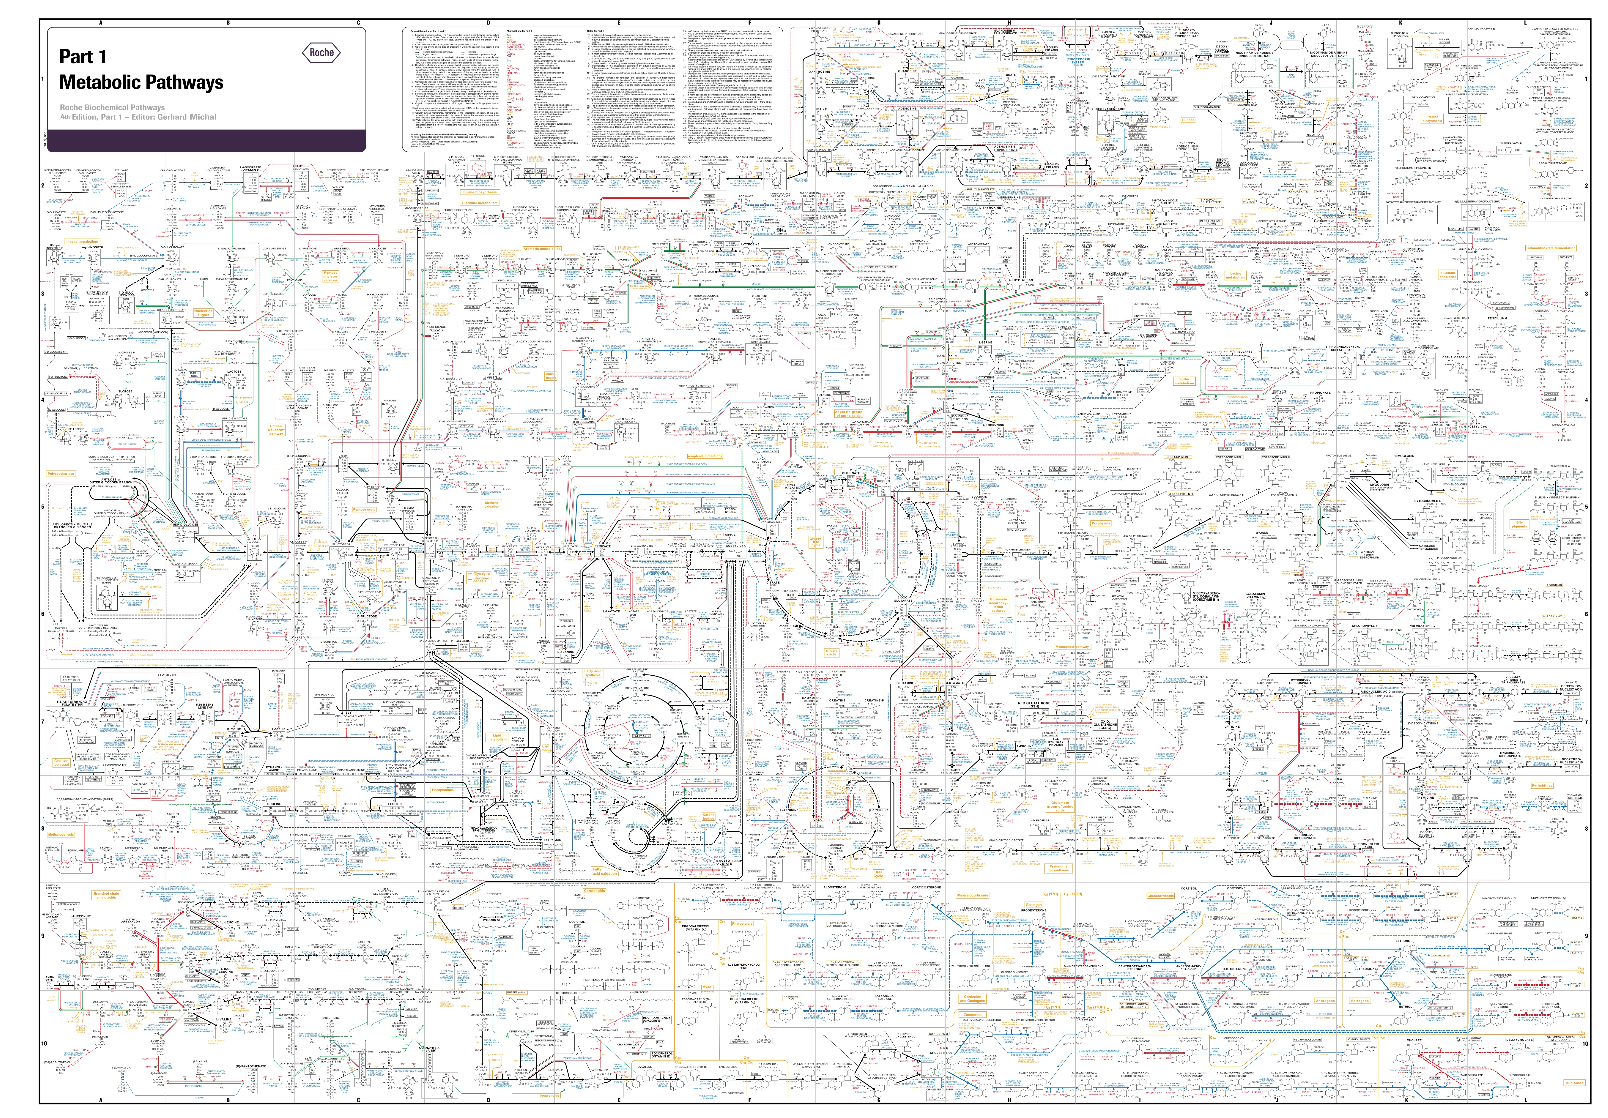
\includegraphics[width=\textwidth]{chem-pics/metabolic-pathways.png}	
	\caption{The Metabolic Pathways poster by Dr. Gerhard Michal from Roche Biochemical \cite{RouchePathways}}
	\label{fig:metabolic-pathways}
\end{figure}

We'll introduce and mathematically define Chemical Reaction Networks (CRN) consisting of:

the set $S = \left\{ X_1, \dots, X_n \right\}, \left| S \right| = n$ of chemical species,

and $r$ reactions of the form:
\begin{equation}\label{mass-action_network}
	\alpha_{1j} X_1 + \dots + \alpha_{n j} X_n \xrightarrow{k_j} \beta_{1j} X_1 + \dots + \beta_{n j}, \forall j = \overline{1,r}.	
\end{equation}

Where $\alpha_{ij}$ is the coefficient of stoichiometry of the reactant $X_i$ in reaction $j$.

The same goes for $\beta_{ij}$, but for the \textbf{produced} $X_i$ in reaction $j$. These are also called the \textbf{stoichiometries} of each reactant / product.

$k_j$ are the reactions' rate constants.

We denote the species' concentrations with $[X_1], \dots, [X_n]$.

We could shorthand both of them in their vector form:
\begin{gather*}
	x \in \mathbb{R}^n_{> 0},  k \in \mathbb{R}^r_{\geq 0} \\
	x =
	\begin{pmatrix}
		x_1 \\
		\vdots \\
		x_n 	
	\end{pmatrix}, \quad k =
	\begin{pmatrix*}
		k_1  \\
		\vdots \\
		k_r	
	\end{pmatrix*}
\end{gather*}
Now we may define the mass-action \textbf{reaction rate} of this particular reaction, which depends on the rate constant, the concentrations of reacting species and their molecularities.
\footcite{Derbez2015,Lorand2024}
\begin{definition}
	\textbf{Reaction Rate}:	
	\begin{align}\label{reaction_rate}
		v : \mathbb{R}^r_{\geq 0}  &\bigtimes \mathbb{R}^n_{> 0} \rightarrow \mathbb{R}_{\geq 0}  \nonumber \\
		v(k,x) &= k_j [X_1]^{\alpha_{1j}} \dots [X_n]^{\alpha_{nj}} \\
		&= k_j x_1^{\alpha_{1j}} \dots x_n^{\alpha_{nj}} \nonumber
	\end{align}
\end{definition}

The way we use such a model for representing chemical reactions is with the premise that the concentrations of the species are not affected by their spatial distribution, so no funky spatial gradients and partial differential equations. Implying the "room" they have is considered necessary, the only factor in the reactions' rate being their "active mass", meaning their concentration or activity.

Otherwise, way more complex models would be used. Ones that take into account things like intermolecular interactions, the mixing process of the solution etc.

A pretty common example that you might've seen in 6th grade would be:
\[
	2H_2 + O_2 \xrightarrow{k} 2H_2O
\]
Where its reaction vector is:
\[
	\bordermatrix{\cr \cr
		H_2 & -2 \cr
		O_2 & -1 \cr
		H_2O & 2 \cr
	}
\]
with reaction rate $v(k,x) = k[H_2]^2[O_2]$. Or, by using the vector $x=(x_1, x_2, x_3, x_4)$: $v(x) = k x_1^2 x_2$.
So the reaction's dynamical system (defined more in detail in \ref{3.2.1}) is:
\begin{align}\label{1st_example_dyn_system}
	\frac{d}{dt}
	\begin{pmatrix*}
		x_1 \\
		x_2 \\
		x_3
	\end{pmatrix*} =
	\begin{pmatrix}
		-2 \\
		-1 \\
		2
	\end{pmatrix}
	v(k,x)
\end{align}
But if we have multiple such reactions we need to use their $\ldots$
\begin{definition}
	\textbf{Stoichiometric matrices.}
	\begin{align*}
		\Gamma_L, \Gamma_R &\in \mathcal{M}_{n \bigtimes r}(\mathbb{N}) \\
		(\Gamma_L)_{ij} &= \alpha_{ij} \text{ from \ref{mass-action_network}} \\
		(\Gamma_R)_{ij} &= \beta{ij} \text{ from \ref{mass-action_network}} \\
		\Gamma &\in \mathcal{M}_{n \bigtimes r}(\mathbb{Z}) \\
		\Gamma &= \Gamma_R - \Gamma_L
	\end{align*}
	$\Gamma_L$ the \textbf{left} stoichiometric matrix, \\
	$\Gamma_R$ the \textbf{right} stoichiometric matrix, and \\
	$\Gamma$ : the \textbf{full} stoichiometric matrix.
\end{definition}
So constructing their equivalent of \ref{1st_example_dyn_system}:
\begin{align}\label{crn_system_matrix_form}
	\frac{d}{dt}
	\begin{pmatrix*}
		x_1 \\
		\vdots \\
		x_n
	\end{pmatrix*} = \Gamma
	\begin{pmatrix*}
		v_1(k,x)	 \\
		\vdots \\
		v_r(k,x)
	\end{pmatrix*}
	\text{ or, even more shorthand:  }
	\frac{dx}{dt} = \Gamma v(k,x).
\end{align}
Where
\begin{definition}\label{flux_vector}
	\textbf{Flux Vector.}
	\begin{align}
		v : \mathbb{R}^r_{\geq 0}  \bigtimes &\mathbb{R}^n_{> 0} \rightarrow \mathbb{R}^r_{\geq 0}  \nonumber \\
		(v(x,k))_{i} &= v_i(k_i, x)
	\end{align}
	is a column vector of all reaction rates for the reactions. For reasons later discussed in \ref{convex_paramteres}, we will call it the \textbf{flux vector.}
\end{definition}

\newpage
\textbf{Example}\label{bigger_network_example1} 1:
One such bigger network would be the following \textbf{open network}.
\begin{align*}
	A + C \xrightarrow{k_{1}} 2A \\
	B + C \xrightarrow{k_{2}} 2B  \\
	A \xrightarrow{k_{3}} \emptyset \\
	B \xrightarrow{k_{4}} \emptyset \\
	\emptyset \xrightarrow{k_{5}} C
\end{align*}
Or, where the last $3$ degradation / production reactions could also be written as
\begin{align*}
	A \xrightarrow{k_{3}} \\
	B \xrightarrow{k_{4}} \\
	\xrightarrow{k_{5}} C	
\end{align*}
To indicate interaction with the "outside" world (kind of like an interface to the outside world).
Here: 	

$C$ is like a "resource" molecule.

$A$, $B$ \textbf{autocatalyze} themselves with $C$, so they produce themselves as they go, until they use $C$ up and one of them ends up on top, depending on their initial concentrations, so this system would also be \textbf{bistable}.

This system would look like:
\begin{align*}
	\Gamma_L =
	\begin{pmatrix}
		1 & 0 & 1 & 0 & 0 \\
		0 & 1 & 0 & 1 & 0 \\
		1 & 1 & 0 & 0 & 0
	\end{pmatrix}
	, \quad
	\Gamma_R =
	\begin{pmatrix}
		2 & 0 & 0 & 0 & 0 \\
		0 & 2 & 0 & 0 & 0 \\
		0 & 0 & 0 & 0 & 1
	\end{pmatrix}
\end{align*}
\begin{equation*}
 \Gamma =
 \begin{pmatrix*}
		1 & 0 & -1 & 0 & 0 \\
		0 & 1 & 0 & -1 & 0 \\
		-1 & -1 & 0 & 0 & 1
 \end{pmatrix*}
\end{equation*}
Whereas, the reaction rate:
\[
	v(k,x) =
	\begin{pmatrix*}
		v_{1}(k,x)	 \\
		v_{2}(k,x)	 \\
		v_{3}(k,x)	 \\
		v_{4}(k,x)	 \\
		v_{5}(k,x)
	\end{pmatrix*} =
	\begin{pmatrix}
		k_1 x_1 x_3 \\
		k_2 x_2 x_3 \\
		k_3 x_1 \\
		k_4 x_2 \\
		k_5
	\end{pmatrix}
\]
And so its dynamical system in matrix form is:
\begin{align*}
	\frac{dx}{dt} &= \Gamma v(k,x) \\
	\frac{d}{dt}
	\begin{pmatrix*}
		x_1	\\
		x_2	\\
		x_3	
	\end{pmatrix*} &=
	\begin{pmatrix*}
		1 & 0 & -1 & 0 & 0 \\
		0 & 1 & 0 & -1 & 0 \\
		-1 & -1 & 0 & 0 & 1
 \end{pmatrix*}
	\begin{pmatrix}
		k_1 x_1 x_3 \\
		k_2 x_2 x_3 \\
		k_3 x_1 \\
		k_4 x_2 \\
		k_5
	\end{pmatrix}
\end{align*}
As you can see this is the same as \ref{1st_example_dyn_system}, I just didn't use the notation " $\Gamma$ " then. This results in:
\[
	\begin{cases*}
		\dot{x}_1 = k_1 x_1 x_3 - k_3x_1  \\
		\dot{x}_2 = k_2 x_2 x_3 - k_4 x_2  \\
		\dot{x}_3 = -k_1 x_1 x_3 - k_2 x_2 x_3 + k_5 \\
	\end{cases*}
\]

\textbf{Interaction graphs}\footcite{Derbez2015}: Every chemical reaction network has its corresponding interaction graph, formed of the following basic structure.

Two intersecting arrows mean a sum of the reacting / produced species.

So for reactions of the form
\begin{align*}
	B + A \xrightarrow{k_{1}} D + C
\end{align*}
Their interaction graph would be:
\usetikzlibrary{arrows.meta, positioning}

\begin{center}
	\begin{tikzpicture}[>=Stealth, node distance=2cm]
		\centering
		\node (B) {B};
		\node[below=1.2cm of B] (A) {A};
		\node[right=3cm of A] (C) {C};
		\node[right=3cm of B] (D) {D};

		\draw[->, bend left=45] (A) to (C);
		\draw[->, bend right=45] (B) to (D);
	\end{tikzpicture}
\end{center}

We'll use these kinds of figures in later chapters, when talking about more specific CRN's.
But one thing that's certain is these CRN's can also be modeled by: \ldots
\chapter{Dynamical Systems}
\label{chap:ch3}

\section{Defining Ordinary Differential Equations}
\begin{definition}
  \textit{An \textbf{ordinary differential equation} is an equation of an unknown function of \textbf{one} variable. This can be expressed as a function \textbf{of} this unknown function, its corresponding variable and its various derivatives}.
\end{definition}
Its general form looks something like:
\begin{equation}\label{ODE}
  F(t,y(t),y'(t),....,y^{(n)}(t))=0,
\end{equation}
Where $y(t)$ is the unknown function of independent variable $t$ and $F : \Omega \rightarrow \mathbb{R},\hspace{0.1cm}\Omega \subseteq \mathbb{R}^{n+1}$. \\
This would be what's called the implicit form of the differential equation.

\begin{definition}
  \textit{The \textbf{order} of an ODE is the highest order of the derivative present in the equation.}
\end{definition}
In our case, the order is $n$.
If, however $F$ satisfies the regularity condition \textbf{of the implicit function theorem} then the equation can be written in a much more digestible form. \\

The \textbf{implicit function theorem} allows one to convert a relation (implicit form) to functions of some variables. These functions may not be unique, but togather, their graph may locally satisfy the relation. \\
As an example: The relation for a cardiod cannot be expressed as a sole function, we'd instead need the union of the graph of two separate functions for expressing it.
(si aici gen faci tu niste graphuri cu maple sau alte d-astea vezi cum faci virtual machineu ala sau mergi la faculta la un pc cu maple si iti faci lista cu ce vrei sa graphuiesti) \\ \\
\textbf{Reminder}: A function $f(x)$ is continuously differentiable if $\exists f'(x)$ and $f'(x) \in C^n$ where $n>=0$

\begin{theorem}
  Let $F:D \subseteq \mathbb{R}^{n+1}\rightarrow\mathbb{R}$ be a continuously differentiale function with the relation that $F(t,y(t),y'(t),....,y^{(n)}(t))=0$. Let us express a point in the set $\mathbb{R}^{n+1} =\mathbb{R}\bigtimes\mathbb{R}^n$ as (t, \textbf{Y}) = $(t, y,y', \dots, y^{ (n) })$ and fix one such point s.t. $F(t, \textbf{Y})=0$.
  So $\exists \square_{(t, \textbf{Y})} \ni U \bigtimes V \subseteq D$ s.t. $F \in C^1(U\bigtimes V)$ and $\frac{\partial F}{\partial y}(t, \textbf{Y}) \neq 0.$ Then this means $ \exists \square_{t} \ni U_0 \subseteq U,
  \square_{\textbf{Y}} \ni V_0 \subseteq V$ and a function $f : U_0 \rightarrow V_0$ s.t. $f(t) = \textbf{Y}$ and $F(t,f(t))=0, \forall t \in U_0; f \in C^1(U_0)$ and $\frac{\partial f}{\partial t_i} = - \frac{\frac{\partial F}{\partial t_i}(t,f(t))}{\frac{\partial F}{\partial y}(t,f(t))}, \forall i = \overline{1,n} , \forall t \in U_0$ and $F \in C^1(U \bigtimes V),K \in N^* \Rightarrow f \in C^K(U_0).$
\end{theorem}

So restricting the domain $\Omega$ to one that allows the implicit form to be represented as a function of the form
\begin{equation}\label{implicit_func_theorem}
  y^{(n)}(t)=f(t,y(t),y'(t),...,y^{(n-1)}(t))
\end{equation}
would yield what's called the \textbf{explicit} form of the ODE. \\

A \textbf{solution} is an expression of the unknown function $y(t)$ which satisfies the relation \\
$y^{(n)}(t) = f(t,y(t),y'(t),\dots,y^{(n-1)}(t))$. A \textbf{general solution} includes all of these functions and usually has some constants of integration in the expression, while a \textbf{particular solution} doesn't have them. \\
A particular solution is usually found if we also have some initial conditions given for the unknown function, like $y(a)=b, y'(a)=c$ for some $a,b,c  \in \mathbb{R}$.
Or, more formally:

\begin{definition}
  A function $y:I \rightarrow \mathbb{R}$ is a solution of the equation \ref{ODE} if the following conditions are met:

  1. $I \subseteq \mathbb{R}$ is nondegeneate interval. ($|I|>1$)

  2. $y \in C^n(I)$ and $(t,y(t), y'(t), \dots, y^{(n)}(t)) \in D_f, \forall t \in I$.

  3. $y^{(n)}(t)= f(t,y(t),y'(t),\dots,y^{ (n-1) }(t)), \forall t \in I$. ( \ref{implicit_func_theorem} is satisfied)

\end{definition}

\section{Forming Ordinary Differential Equation systems}
We may take a sequence of such first order ordinary differential equations to form a system:

\begin{equation}\label{3.2.1}
  \begin{cases}
    y'_1(t) = f_1(t,y_1(t),y_2(t),\dots,y_n(t)) \\
    y'_2(t) = f_2(t,y_1(t),y_2(t),\dots,y_n(t)) \\
    \vdots                                      \\
    y'_n(t) = f_n(t,y_1(t),y_2(t),\dots,y_n(t))
  \end{cases}
\end{equation}

Constructing $y: D \subseteq \mathbb{R} \rightarrow \mathbb{R}^n, f : D_f    \subseteq \mathbb{R}^{n+1} \rightarrow \mathbb{R}^n$ and denoting \\
$y(t)= (y_1(t), \dots, y_n(t))$ and $f(t,y_1(t),\dots,y_n(t)) = (f_1,\dots,f_n) $ we get what is called the \textbf{ vector form} of the system \ref{3.2.1}.

\begin{equation}\label{3.2.2}
  y'(t) = f (t, y(t))
\end{equation}

\begin{definition}
\end{definition}
For a function $y:D \subseteq \mathbb{R} \rightarrow \mathbb{R}^n$ , $|D| > 1$, if $y \in C^1(D,\mathbb{R}^n)$, and $y'(t) = f(t,y(t)), \forall t \in D \Rightarrow$ $y$ is a \textbf{solution of the system} \ref{3.2.2}.

\begin{definition}
  An \textbf{autonomous equation} is a differential equation that does not explicitly depend on time, but is instead only defined by the relation between the function itself and its derivatives, so an equation of the form
  \begin{equation}\label{eq:3.2.3}
    f(y^{(n)}(t), y^{(n-1)}(t), \dots, y(t))= 0
  \end{equation}
  That is not to say, the function itself does not depend on time, but rather the independent variable $t$ does not explicitly appear in the equation.
\end{definition}

One more famous such example is the equation for the damped oscillator
\begin{equation}\label{eq:3.2.4}
  \ddot{x} + 2\gamma\dot{x} + \omega^2x = 0.
\end{equation} \\
Where \\
\begin{itemize}
  \item $\gamma$ is the damping factor, meaning how quickly the oscillations of the system decay due to loss of momentum (caused by air resistance or friction) \\

  \item  $\omega$ represents the angular (natural) frequency the oscillator would have, were it not to be affected by damping, defined by
    $\omega = \sqrt{\frac{k}{m}}$; where $k$ is the \textbf{elastic stiffness coefficient} of the spring and $m$ the mass. \\
\end{itemize}

In addition, a frequently used notation in physics is
$\dot{x} = \frac{d}{dt}x$ , $\ddot{x}=\frac{d^2}{dt^2}x$
\\

That equation is a \textbf{linear} homogenous equation with constant coefficients (hence autonomous), which is pretty nice to work with. Their general form would be:

\begin{equation}\label{lin_hom_eq_const}
  x + a_1\dot{x}+ \dots +a_{n} x^{(n)} = 0
\end{equation}

Finding exact solutions, though, can be done by using some nice properties of Euler's exponential function $e^{rt}$.

Introducing the notion of \textbf{operators} would help in writing this next section.

\begin{definition}
  $D = \frac{d}{dt}$ is the \textbf{derivation operator}:
  $D^n = \frac{d^n}{dt^n}$, so $D^nu = D^n(u) =\frac{d^nu}{dt^n}$ where $u=u(t)$
  \par
  \hspace{20pt} and (related to \ref{lin_hom_eq_const}): \par
  \hspace{20pt} $L = 1 + a_1D + \dots + a_nD^n$ \par
  \hspace{20pt} is the \textbf{linear differential operator of order n}. Meaning \ref{lin_hom_eq_const} $\iff Lx=0$.
\end{definition}

We now can; just by pure Ansatz; assume the solutions take the form $e^{rt}$ for some (yet unknown) $r$'s. Because the exponential is so easy to work with when it comes to taking derivatives - a.k.a. : $D^n(e^{rt})=r^ne^{rt}$, so its derivatives are proportional to itself, meaning no new $t$'s are introduced - substituting back into \ref{lin_hom_eq_const} yields
\begin{gather*}
  Le^{rt} = e^{rt} + a_1 De^{rt} + \dots +a_{n} D^ne^{rt} = 0      \\
  \Updownarrow \\
  e^{rt}+a_1re^{rt} + \dots + a_nr^ne^{rt} =0 \\
  \Updownarrow \\
  1 + a_1r + \dots + a_nr^n =0
\end{gather*}
The left-hand-side is the \textbf{characteristic polynomial} of the linear equation.
\[
  p(r) = 1 + a_1r + \dots + a_nr^n
\]
Notice that $L = p(D)$. \\
So now it all comes down to finding its roots $r$.

Case \rom{1}: A \textbf{unique, real} root found:

now $e^{rt}$ is a \textbf{fundamental solution} for $Le^{rt}=0$ \par
\newpage
Case \rom{2}: A \textbf{unique, complex} root found:

say it has the form $r = \lambda \pm i\mu, \mu \neq 0$. \\
By Euler's formula:
\begin{equation}\label{euler}
  e^{rt} = e^{(\lambda + i\mu)t} = e^{\lambda t} \cdot e^{i \mu t}  =  e^{\lambda t} \cdot [\text{cos}(\mu t) + i \text{sin}(\mu t)]
\end{equation}

So $e^{\lambda t}\text{cos}(\mu t)$ and $e^{\lambda t}\text{sin}(\mu t)$ are both fundamental solutions for $Lx=0$.\\

\textbf{Proof}: \par
Since $a_i \in \mathbb{R}, \forall i=\overline{1,n}$ in $p \implies p(\overline{r})=\overline{p(r)}, \forall r \in \mathbb{C}$, hence, just like 2AM coffee and the exam session, complex roots of $p$ always come in pairs. They both satisfy:
\begin{equation}\label{lin_op_solution}
  Le^{(\lambda \pm i \mu)} = 0
\end{equation}

But since our $x : \mathbb{R} \rightarrow \mathbb{R}$ we're looking for \textbf{real} valued solutions.
Because $\mu \in \mathbb{R}$ the following properties hold equivalently for $\lambda + i\mu$ and for $\overline{\lambda + i\mu}=\lambda - i\mu$ so I'll only write $\lambda \textbf{+} i \mu$ for simplicity.
By \ref{euler}:
\begin{equation}\label{eulers_real_and_imaginary}
  \text{Re}(e^{rt})=e^{\lambda t} \cdot \text{cos}(\mu t), \hspace{2cm}    \text{Im}(e^{rt}) = e^{\lambda t} \cdot \text{sin}(\mu t).
\end{equation}
But (\textbf{reminder})
\begin{gather}\label{real_imag_another_way_to_write}
  \text{Re}(c)= \frac{c+\overline{c}}{2}, \hspace{2cm}
  \text{Im}(c) = \frac{c-\overline{c}}{2i}
\end{gather}
\begin{gather*}
  \forall c \in \mathbb{C}
\end{gather*}

\newcommand\firstConclusion{\stackrel{\mathclap{\normalfont\mbox{\ref{eulers_real_and_imaginary}, \ref{real_imag_another_way_to_write}}}}{=\joinrel=\joinrel=\joinrel=\joinrel=\joinrel=}}

\newcommand\byDistributivity{\stackrel{\mathclap{\normalfont\mbox{dist.}}}{=\joinrel=\joinrel=}}

\newcommand\operatorSatisfy{\stackrel{\mathclap{\normalfont\mbox{\ref{lin_op_solution}}}}{=\joinrel=}}

Using these three conclusions we get:
\begin{align*}
  L(e^{\lambda t} \cdot \text{cos}(\mu t)) \firstConclusion
  L\left(\frac{e^{rt}+e^{\overline{r}t}}{2} \right) \byDistributivity
  \frac{1}{2} \left( Le^{rt} + Le^{\overline{r}t} \right) \operatorSatisfy 0 , \\
  L(e^{\lambda t} \cdot \text{sin}(\mu t)) \firstConclusion
  L\left(\frac{e^{rt}-e^{\overline{r}t}}{2i} \right) \byDistributivity
  \frac{1}{2i} \left( Le^{rt} - Le^{\overline{r}t} \right) \operatorSatisfy 0 ,
\end{align*}

In conclusion,if $Le^c=0$ for some $c \in \mathbb{C} \implies L\text{Re}(e^c)= L\text{Im}(e^c)=0, \text{for } \text{Re}(e^c), \text{Im}(e^c) \in \mathbb{R}$.
Moreover, the same can be said for $e^{\overline{c}}$. \qed \\

Now something let's say ... \textbf{fundamental} (hehe) about these solutions, is they have to be linearly independent to eachother. Meaning the only solution for
\begin{equation}\label{liniar_independece}
  c_1 x_1+c_2 x_2 + \dots + c^n x^n = 0
\end{equation}
is the trivial solution $c_1=c_2=\dots=c_n=0$ where $x_i$ are the fundamental solutions of the system.

So the reson I've emphasized "\textbf{unique}" in the first 2 cases was because If we're to apply those methods for \textbf{repeating} roots, meaning the ones with multiplicity $k>1$, the resulting solutions wouldn't hold \ref{liniar_independece} because they would in fact be the same! \\

To counteract this issue, the clever people over at the 1748 Berlin Academy (just Euler) came up with yet another (easily provable) Ansatz: just multiplying by powers of $x$. \\

A root with multiplicity $k$ would introduce yet another $k$ -for real- or $2k$ - for complex - fundamental solutions to this equation, so to finish what we've started:\\

Case \rom{3}: \textbf{Repeated, real} roots $r$ with multiplicity $k>1$ yield the fundamental solutions \\ $e^{rt}, xe^{rt}, \dots,x^{k-1}e^{rt}$. \\
These can be verified that they do, in fact satisfy \ref{liniar_independece}. So can: \\

Case \rom{4}: \textbf{Repeated, complex} roots $r$ with multiplicity $k>1$. These introduce the pairs:
\begin{align*}
  e^{at}\text{cos}(bt), \ \  e^{at}\text{sin}(bt)  \\
  xe^{at}\text{cos}(bt), \ \ xe^{at}\text{sin}(bt) \\
  \vdots                                           \\
  x^{k-1}e^{at}\text{cos}(bt), \ \ x^{k-1}e^{at}\text{sin}(bt)
\end{align*}

So $2k$ new solutions.

\textbf{The superposition principle} \\
Bernoulli (to the disbelief of Euler and Langrange) told us that the complex behaviour of vibrating strings can be modeled by sepparating their motion into well-defined and easy to compute simple waves with known frequences and amplitudes, which can later be \textbf{superposed} with one-another to form the complete system.
\\

This principle can be applied to \textit{our} easier to compute \textbf{fundamental solutions} ($x_1,\dots,x_n$) in relation to the system formed by our linear operator $Lx =0 $.
\\

Since it's a linear operator, additivity and homogeneity apply:
\begin{gather*}
  L(x_1+x_2) = Lx_1 + Lx_2\\
  aLx = L(ax) , \forall a \in \mathbb{C}
\end{gather*}
where $x,x_1,x_2$ are fundamental solutions of the system.\\
Hence the complete, final, \textbf{general} solution for \ref{lin_hom_eq_const} are linear combinations of all our previously found fundamental solutions:
\[
  x(t) = c_1 x_1 + \dots + c_nx_n
\]
for some constants $c_i$.

\section{Formally defining and characterizing dynamical systems}
The reason why autonomous equations are so useful to us is because of the ease with which we can visualize the \textbf{ evolution} of a system of such equations.
Take, for example:
\begin{definition}

  A \textbf{ system of first-order autonomous equations} is a system of equations of the form

  \begin{equation}\label{fo_system_auton_eq}
    \begin{cases}
      \dot{y}_1 = f_1(y_1,\dots, y_n) \\
      \dot{y}_2 = f_2(y_1,\dots, y_n) \\
      \vdots                          \\
      \dot{y}_n = f_n(y_1,\dots, y_n) \\
    \end{cases}
  \end{equation}

\end{definition}

\begin{definition}
  We can construct the \textbf{phase space} of the \ref{fo_system_auton_eq} dynamical system by:

  \begin{enumerate}
    \item Representing all possible values of $y_i$, $ i = \overline{1,n}$ as points in Euclidean space $S \subseteq \mathbb{R}^n$

    \item Constructing a function $f : S \rightarrow S, f(y_1,y_2,\dots,y_n) = (\dot{y}_1,\dot{y}_2,\dots,\dot{y}_n)$ that attaches to each point in $S$ a vector representing the direction in which to go such that the relation \ref{fo_system_auton_eq} is satisfied.

  \end{enumerate}
\end{definition}

Thus, the \textbf{phase space} of the system is a vector field where $f$ is a continuous vector valued function.\\

So keeping this in mind, we may form a formal definition:\\

\begin{definition}
  A \textbf{dynamical system} is a tuple $(T,S,\Phi)$ where: \\

  \begin{itemize}
    \item $T$: part of the $(T,+)$ monoid of all possible $time$ moments of our system
    \item $S$: is the set of all possible states,and
    \item the function: $\Phi : U \subseteq (T \times S ) \rightarrow S$ where values of the second component span all of $S$, meaning $proj_2(U) = S$.
  \end{itemize}
  In order to give the necessary properties of $\Phi$ we will need to also define: \\
  $I(s):= \{ t \in T | (t,s) \in U \}, \forall s \in S $\\

  so $\Phi$ has the properties that:

  $\Phi(0,s) = s$

  $\Phi(t_2,\Phi(t_1,s)) = \Phi(t_1+t_2,s); \forall t_1, t_1+t_2 \in I(s), t_2 \in I(\Phi(t_1,s)), s \in S$.

  We call such a function $\Phi$ the \textbf{evolution function} of the dynamical system, mapping every state and $time$ after which that specific state is found, to another unique state.
\end{definition}

If we take a specific state $s$ as an initial constant, we can form the function

$\Phi_s : I(s) \rightarrow S$ \\
called the \textbf{flow} through $s$, whose image:

$\gamma_s:=\{\Phi_s(t) | t\in I(s) \}$

is the \textbf{orbit} through $s$,
which is a curve of parameter $t \in I(s)$ representing the values the dynamical system will take throughout the experiment's timespan, given the initial condition (state) $s$.

\hspace{20 mm}

Since a point only belongs to one orbit, if we form the set \par

$\Gamma_{U,\Phi}:=\{ \gamma_s | s \in S \}$  \\
of all orbits of the dynamical system $(U,\Phi)$, with $U\subseteq (T \times S)$ and $\Phi$ the evolution function, it follows that: \\
$\forall \gamma_1,\gamma_2 \in \Gamma_{U, \Phi}, \gamma_1 \bigcap \gamma_2 = \emptyset$, meaning the set of orbits forms a partition of the phase space $S$
\hspace{20 mm}
\\
\textbf{Proof:}
Conditions for partitions:
\par  \textbf{Reminder:} A partition $\Gamma_U$ of a set $U$ is a set of non-empty disjoint subsets of $U$ s.t.

\[
  \bigcup_{\gamma\in \Gamma_U} \gamma = U
\]

So we need to prove:\\

TODO: te apuci de asta mai incolo \par
\rom{1}. $\gamma \subseteq U, \forall \gamma \in \Gamma_{U,\Phi}$ \par
\rom{2}. $ \gamma \neq \emptyset, \forall \gamma \in \Gamma_{U,\Phi}$ \par
\rom{3}. $\gamma_1 \bigcap \gamma_2 = \emptyset, \forall \gamma_1, \gamma_2 \in \Gamma_{U,\Phi}$ \par
\rom{4}. $\bigcup_{\gamma\in \Gamma_U} \gamma = U$ \par
\vspace{5mm}

TODO: oki, deci aici zici cum se rezolva o ecuatie autonoma liniara in mod normal si despre solutiile fundamentale si independenta si dependa lor and stuff si dupa dai un mod echivalnt de a le rezolva cu metoda de mai jos care face un sistem din ele

We may, in fact construct an equivalent system

\[
  \begin{cases}
    \dot{y}_1 = f_1(y_1,\dots, y_n) \\
    \dot{y}_2 = f_2(y_1,\dots, y_n) \\
    \vdots                          \\
    \dot{y}_n = f_n(y_1,\dots, y_n) \\
  \end{cases}
\]

Starting from any autonomous differential equation

\[
  f(y^{(n)}(t), y^{(n-1)}(t), \dots, y(t))= 0
\]

via a technique which associates to each respective derivative a state unknown (variable).
This system's form depends on the solvability with respect to the highest derivative $y^{(n)}$. \\
The first form may be obtained if the above equation \textbf{can} be solved in terms of $y^{(n)}$, meaning it can be re-written as
\begin{gather*}
  f(y^{(n)}(t), y^{(n-1)}(t), \dots, y(t))= 0 \\
  \Updownarrow \\
  y^{(n)}  = G(y^{(n-1)}(t), \dots, y(t))
\end{gather*}

We first take each state unknown to be equal to their respective derivatives, so:
\begin{gather*}
  y_1 = y     \\
  y_2 = \dot{y} \\
  \vdots \\
  y_n = y^{(n-1)}
\end{gather*}

Then we take the derivatives with respect to time of each of these equations, so starting with $\dot{y}_1 = \dot{y}$, but $\dot{y} = y_2$, so $\dot{y_1}=y_2$. Continuing on like that, in a sort of diagonal fashion, we get:
\begin{gather*}
  \dot{y}_1 = y_2 \\
  \dot{y}_2 = y_3 \\
  \vdots \\
  \dot{y}_{n-1} = y_n \\
\end{gather*}
and this is where that beginning "solvability" part comes into play. The very last one will be exactly its solution defined earlier:
\[
  \dot{y}_n = \frac{d}{dt}y^{(n-1)} = y^{(n)}  = G(y^{(n-1)}(t), \dots, y(t))
\]

So, putting this all together we can get the equivalent system of the autonomous differential equation
\[
  \begin{cases}
    \dot{y}_1 = y_2     \\
    \dot{y}_2 = y_3     \\
    \vdots              \\
    \dot{y}_{n-1} = y_n \\
    \dot{y}_n  = G(y^{(n-1)}(t), \dots, y(t))
  \end{cases}
\]

Now, if instead of an actual function $G$ we only get an implicit form for a solution (\ref{implicit_func_theorem} isn't satisfied), we could write the original equation in terms of these new state variables:

\begin{gather*}
  f(y(t), \dot{y}(t),\dots,y^{(n-1)},y^{(n)})= 0 \\
  \Updownarrow \\
  f(y_1,\dots,y_n,\dot{y}_n) = 0
\end{gather*}

So the system would be:

\[
  \begin{cases}
    \dot{y}_1 = y_2     \\
    \dot{y}_2 = y_3     \\
    \vdots              \\
    \dot{y}_{n-1} = y_n \\
    f(y_1,\dots,y_n,\dot{y}_n) = 0
  \end{cases}
\]

This is a differential-algebraic system of equations (DAE), which is beyond the scope of this thesis but figured I'd cover all cases (this one's usually solved via numerical methods).

\vspace{10pt}

Okay, but now since we know how to form systems from any autonomous equation \dots how does that make our lives easier in any way?

Let's consider \ref{lin_hom_eq_const}, the equation we worked with previously. Now we can express it differently:

we could first divide everything by $a_{n}$ so everything looks a bit better.

\begin{gather*}
  \left. a_0 x + a_1\dot{x}+ \dots +a_{n} x^{(n)} = 0 \middle| \frac{1}{a_{n}} \right. \\
  \Updownarrow \\
  b_0 x + b_1\dot{x} + \dots + b_{n-1} x^{(n-1)} + x^{(n)} = 0
\end{gather*}

And now apply the aforementioned technique:

\begin{gather*}
  x_1 = x     \\
  x_2 = \dot{x} \\
  \vdots \\
  x_n = x^{(n-1)}
\end{gather*}

then:

\[
  \begin{cases}
    \dot{x}_1 = x_2     \\
    \dot{x}_2 = x_3     \\
    \vdots              \\
    \dot{x}_{n-1} = x_n \\
    \dot{x}_n  = x^{(n)} = -b_0x - b_1\dot{x} - \dots - b_{n-1} x^{(n-1)} = -b_0 x_1 - b_1 x_2 - \dots - b_n x_{n-1}
  \end{cases}
\]

Waitt, I saw this somewhere in year 1, semester 1 during Linear Algebra (which I definitely didn't have to re-take twice)

That is the same as:
\begin{align*}
  \begin{bmatrix}
    \dot{x}_1     \\
    \dot{x}_2     \\
    \dot{x}_3     \\
    \vdots        \\
    \dot{x}_{n-1} \\
    \dot{x}_n
  \end{bmatrix} =
  \bordermatrix{ & x_1    & x_2    & x_3    & \ldots & x_n \cr
    & 0      & 1      & 0      & \ldots & 0 \cr
    & 0      & 0      & 1      & \ldots & 0 \cr
    & 0      & 0      & 0      & \ldots & 0 \cr
    & \vdots & \vdots & \vdots & \ddots & \vdots \cr
    & 0      & 0      & 0      & \ldots & 1 \cr
  & -b_0   & -b_1   & -b_2   & \ldots & b_n }
  \begin{bmatrix}
    x_1     \\
    x_2     \\
    x_3     \\
    \vdots  \\
    x_{n-1} \\
    x_n
  \end{bmatrix}
\end{align*}

care poate fi gen rezolvat sa-i gasest eigen valusurile pe care le folosesti cu solutiile fundamentale sa gasesti eigenvectorsii respectivi pt eigenvalurieile alea si poti astfelll gen sa-ti dai seama stabilitatea sistemului => stabilitatea ecuatiei de la care ai plecat din prima gen.

//TODO:1. prima data dai exemple de sisteme liniare si cum fac ecuatiile diferentiale sa se pupe cu algebra liniara si de toate felurile in care poti sa rezolvi algebreic sisteme de ecuatii diferentiale ,eigenvalues eigenvectors din astea \par
2. SI dupaa zici okay but what if my system is not linear? \textbf{Then} how will forming its corresponding system help me? Si dai exemplul cu pendumulul, reintroducand idea de phase space si cum poti sa-l formezi tu acum folosind metoda de mai sus (o sa-i dau un nume mai incolo s-o referentiezi)

Taking, in particular, a more complex autonomous differential equation; the one for the damped pendulum:

\begin{equation}\label{damped_pendulum}
  \ddot{\theta} +\mu\dot{\theta} + \frac{g}{L}\sin(\theta) = 0
\end{equation}
where:  \par
$
\left.
\begin{array}{l}
  \theta : \text{angular position}       \\
  \dot{\theta} : \text{angular velocity} \\
  \ddot{\theta} : \text{angular acceleration}
\end{array}
\right\}
\text{all functions of } t \text{ (time)}
$

\ \ $\mu = \frac{c}{mL}$ : dampening factor \par
\ \ $c$ : the dampening coefficient due to the resistive forces \par
\ \ $m$: mass at the end of the pendulum \par
\ \ $g \approx 9.81 \frac{m}{s^2}$: earth's gravitational acceleration \par
\ \ $L$: the pendulum's length \par

We can express $\theta$ and $\dot{\theta}$ as two separate and independent variables in a 2D space of points \par $(\theta,\dot{\theta}) = (\theta,\omega)$.
And attach to each point the vector formed from the derivatives of each component, which would be (according to \ref{damped_pendulum}):

\begin{align}
\frac{d}{dt}
\begin{bmatrix}
  \theta \\
  \dot{\theta}
\end{bmatrix} =
\begin{bmatrix}
  \dot{\theta} \\
  \ddot{\theta}
\end{bmatrix} =
\begin{bmatrix}
  \omega \\
  -\mu \cdot \omega - \frac{g}{L}\sin(\theta)
\end{bmatrix}
\end{align}

This would in turn form the phase portrait of the dynamical system, described by a system of first-order autonomous differential equations:

\[
\begin{cases}
  \dot{\theta}  = \omega \\
  \dot{\omega} = -\mu \cdot \omega - \frac{g}{L}\sin(\theta)
\end{cases}
\]

\par
TODO: faci tu dupa aici un plot in matlab frumusel
si dupa mai gasesti un exemplu mistio in 3d

arat dupa ce faci toate demonstratiile pentru n dimensiuni, niste poze si cazuri particulare in 2,3 dimensiuni, cv ce se paote vedea cu poze

4. arata in state spaceu ala cum iti dai seama stabilitatea sistemului dand graficul oribtelor in vector spaceu ala ( sa mai pui si snite poze)\\

We can observe that the pendulum will not move an inch if it is just left in its "equilibrium" point hanging down ($\omega \equiv \theta \equiv 0$), but that like a coin left on its side, it will also stay still if started at the \textbf{polar} opposite angle in relation to the stability angle ($\omega =0 , \theta = 180 \degree)$, standing up.
Althought, like a coin left standing on its side, even the slightest deviation will get it tumbling down. This can be observed in the system's phase portrait. The study of how much such changes in initial conditions influence later behaviour is what we call the \textbf{stability} of certain points inside the system.

5. arata poza de clasificarea sistemelor, dat \\

\chapter{Existence and Absence of Hopf Bifurcation in Phosphorylation-Dephosphorylation CRN}

\section{What even \textbf{is} a bifurcation?}
To better generalize them, it'd be best to also define the notion of:

\begin{definition}
	\textbf{Invariant sets}.

	Taking the Auton. sys.
	\begin{equation}\label{invar_set_auton_sys}
		\dot{y} = f(y) , y(0) = y_0, y \in \mathbb{R}^n
	\end{equation}

	A state-set $S \subseteq \mathbb{R}^n$ of \ref{invar_set_auton_sys} is \textbf{invariant} if $\forall y_0 \in S, \forall t \geq 0: y(t) \in S$
\end{definition}

As you can see by this above definition, equilibria are also particular cases of invariant sets, themselves.

They also fall into stability classes that can be defined as in Def. \ref{equilibrium_stability}, but replacing
\[
	"y_0" \text{ with } "S \subseteq \mathbb{R}^n \text{ }"
\]
and
\[
	" \dotso \norm{y(t) - y_0} \dotso" \text{ with } "\dotso \text{ inf}\{ \norm{y(t) - s} : s \in S  \} \dotso \text{ }"
\]
The Jacobian (linearization), generally, would also not be as useful in this context anymore.
\newpage
Now consider we have a system as above, except it now depends on an extra parameter $\mu$, which remains constant \textbf{during} our "experiment".
\begin{equation}\label{auton_parameter_sys_compact}
	\dot{y} = f_\mu(y).
\end{equation}

This could be, for example, the length of the pendulum $L$, in \ref{damped_pendulum}, or its damping coefficient $c$. Honestly generalizing it even more, it could even be the gravitational constant $g$. Hence, this parameter can, of course be a \textbf{vector} of such parameters.

The way the parameter $\mu$ varies also induces variations in the topology and dynamics of the system. That's obvious since this is kind of the point of parameters in systems.

What can vary though can be trivial or more interesting.

The positions of invariant sets, for example can vary continuously

during changes in $\mu$; that's usually normal.

But what's more interesting is when these change their \textbf{stability} altogether, equilibria disappear completely / appear out of thin-air - or, even - collide with other invariant sets.

This odd behavior is called a \textbf{bifurcation}, and $\mu$, in this case is a \textbf{bifurcation parameter}.

The former types of bifurcations I talked about previously are called \textbf{local}, those in which changes in stability can only be considered mostly for \textbf{isolated equilibria}, individually, or other invariant sets whose stability can be analyzed \textbf{locally}, via the system's linearization at a point.

The latter are \textbf{global}, which are more complex and require greater understanding of the system beyond a local linearization, but that falls into the special-case category described in the last paragraphs of the previous chapter, and so far all I know about Mr. Prof. Lyapunov as of now is that his brother was pianist. But thankfully our interest for this work lies with local bifurcations, so we'll be ignoring this for now, maybe I'll come back to it during my Master's (not).

To better define and illustrate them for the 1-D case and give example of bifurcations for such dimension, we could instead write our vector field $f$ as depending on $\mu$ in addition to the unknown function $y$.
\begin{equation}\label{eq:1-d_bif_sys}
	\dot{y} = f(y, \mu).
\end{equation}
And assume $f \in C^k(\mathbb{R} \bigtimes \mathbb{R}), k \geq 2 $ around $(0,0)$, and
\begin{equation}\label{bifurcation_priming}
	f(0,0) = 0, \quad \frac{\partial f}{\partial y}(0,0) = 0.
\end{equation}
By these conditions we are basically "priming" the system for bifurcations, but none are enough for them to actually occur. Here come the specific definitions for each particular type of bifurcation in 1-D.

\begin{definition}
	A \textbf{Saddle-node bifurcation}:
	for $f$ in \ref{bifurcation_priming}, add as well:
	\begin{equation*}
		\frac{\partial f}{\partial \mu}(0,0) =: a \neq 0, \quad \frac{\partial^2 f}{\partial y^2}(0,0) =:b \neq 0.
	\end{equation*}
\end{definition}
Then, for \ref{eq:1-d_bif_sys}, a saddle-node bifurcation occurs at $\mu = 0$, if the following equivalences are true:

\rom{1}. For $ab < 0$ (resp. $ab> 0$), $\nexists y : f(y,\mu) = 0$ for $\mu < 0$ (resp. $\mu > 0$)

\rom{2}. For $ab < 0$ (resp. $ab > 0$), $\exists y_+(\epsilon) \neq y_-(\epsilon) \implies y_\pm(\epsilon) : f(y_\pm(\epsilon), \mu) = 0, \epsilon = \sqrt{\abs{\mu}}$, for $ \mu > 0 $ (resp. $\mu < 0$), having opposing stabilities.

\begin{definition} \label{pitchfork_bif}
	\textbf{Pitchfork bifurcation}.

	For $f$ from \ref{bifurcation_priming}, assume as well that:
	$f \in C^k, k \geq 3$,
	\[
		f(-y, \mu) = -f(y,\mu)
	\]
	and,
	\[
		\frac{\partial^2 f}{\partial \mu \partial y}(0,0) =: a \neq 0, \quad \frac{\partial^3 f }{\partial y^3}(0,0)=: b \neq 0
	\]

	Now, a \textbf{pitchfork bifurcation} occurs for \ref{eq:1-d_bif_sys} at $\mu  =0$ if:

	\rom{1}. for $ab < 0$ (resp. $ab > 0$) $\exists! y = 0 :f(y,\mu) = 0 $ for $\mu < 0$ (resp. $\mu > 0$). $b < 0 \implies$ stable, $b > 0 \implies$ unstable.

	\rom{2}. for $ab < 0$ (resp. $ab > 0$) $\exists y = 0 : f(y , \mu) = 0$, as well as: $y_+(\epsilon) \neq y_-(\epsilon) \implies y_\pm(\epsilon) : f(y_\pm(\epsilon), \mu) = 0, \epsilon = \sqrt{\abs{\mu}}$  for $\mu > 0$ (resp. $\mu < 0$), for which $y_+(\epsilon) = -y_-(\epsilon)$, Both $y_-(\epsilon)$ and $y_+(\epsilon)$ have matching stabilities, whereas $y = 0$ has the opposite stability of them, given by $b < 0 \implies$ stable, $b > 0 \implies$ unstable.
\end{definition}

\begin{definition}
	\textbf{Transcritical bifurcation}.

	For $f$ in \ref{bifurcation_priming}:
	\[
		\frac{\partial^2 f}{\partial \mu \partial y}(0, 0) =:a \neq 0, \quad \frac{\partial^2 f}{\partial y^2}(0,0) =: b \neq 0
	\]
	Then a \textbf{transcritical bifurcation} occurs for \ref{eq:1-d_bif_sys} at $\mu = 0$, char. by (if they hold):

	\rom{1}.  $\exists y = 0 : f(y, \mu) = 0$  and  $ \exists y_0(\mu) : f(y_0(\mu), \mu) = 0 $ where $\mu \rightarrow u_0(\mu) \in C^m, m = k - 2$

	\rom{2}.  for $a\mu  < 0$ (resp. $a\mu > 0$) the trivial fixed point $y = 0 \implies$ stable (resp. unstable)
	and $u_0(\mu)$ has opposing stability.
\end{definition}

Finding local bifurcations can be done by looking at eigenvalues.
\newpage
{\large The local bifurcation condition

}For system:
\begin{equation}
	\dot{y} = f(y, \mu) \quad f : \mathbb{R}^n \times \mathbb{R} \rightarrow \mathbb{R}^n
\end{equation}

\begin{definition}\label{local_bif_def}
	$(y_0,\mu_0)$ admits a \textbf{local bifurcation} if:
\end{definition}

If $\forall \lambda \in Eig(J_{f}(y_0,\mu_0)) : Re(\lambda) \leq 0$, while $\exists \lambda_0 : Re(\lambda_0) = 0$

\begin{equation}\label{stable_state_bif}
	\text{If } \lambda_0 = 0 \text{ the bifurcation is stable-state defined. }
\end{equation}

We also have a second kind of local bifurcation and this is where we begin the crux of the thesis, and answer the first question I had getting into this:

\section{What is a simple Hopf Bifurcation?}

A \textit{simple Hopf bifurcation} is a bifurcation in which a single complex-conjugate pair of eigenvalues of the Jacobian matrix crosses the imaginary axis, while all other eigenvalues remain with negative real parts. Such a bifurcation generates nearby oscillations or periodic orbits.

Or, more formally, defined similarly to Def. \ref{local_bif_def}:
\begin{definition}
	$(y_0, \mu_0)$ admits a \textbf{Hopf bifurcation} if we have Def. \ref{local_bif_def}, and additionally:
	\begin{equation}\label{hopf_bif_def}
		\exists! \lambda_0 : Re(\lambda_0) = 0, \quad
		Im(\lambda_0) \neq 0.
	\end{equation}
\end{definition}
Visually, just to hammer it in:

\begin{figure}[H]
	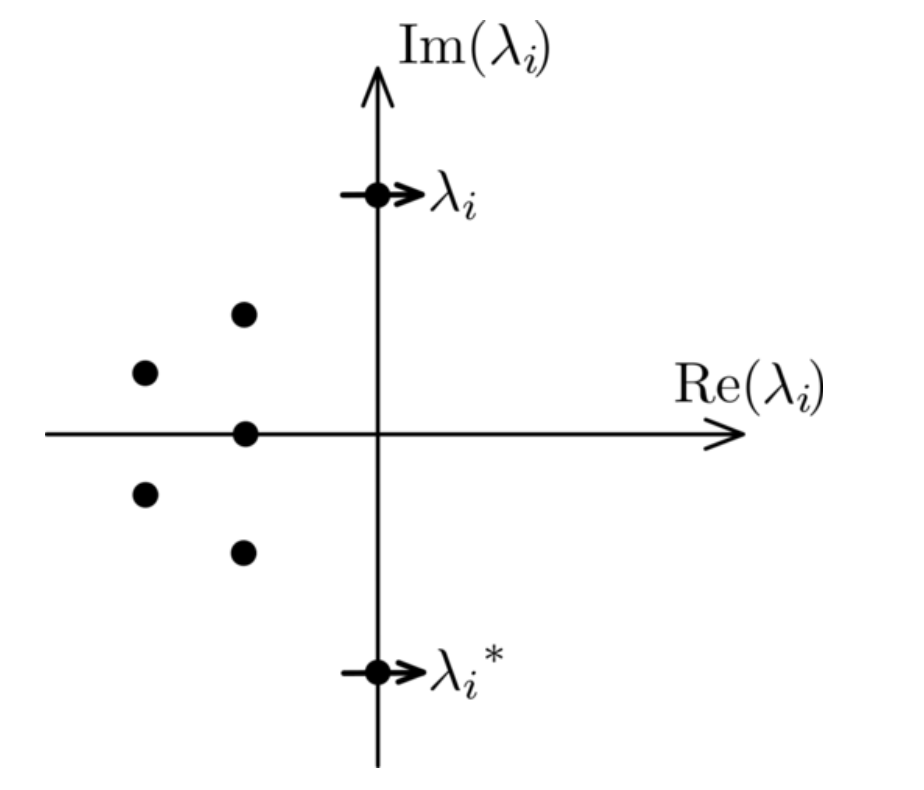
\includegraphics[width=13cm]{math_pics/hopf-bif-eigenvalue-graph.png}
	\centering
	\caption{Visualizing the zeroes}
\end{figure}

In $\mathbb{R}^2$, such Bifurcations cause special kinds of invariant sets, namely \textbf{limit cycles} to appear. These are periodic solutions, for which we'll need a few more concepts in order to be able to define them:
\begin{definition} \textbf{Closed trajectory and Closed orbit (cycle)}

	A trajectory (or flow): $y(t) \in \mathbb{R}^2$ as in Def. \ref{dyn_sys_orbit_flow_etc_def} is a solution for \ref{eq:1-d_bif_sys}

	A closed trajectory is one which returns to its starting point $\forall s_0 := \Phi(0,s) $ it has, namely:
	\begin{gather*}
		\exists t_0 \in T : \Phi(t,s) = \Phi(t+t_0,s), \forall s \in \Phi_{s_0}     \\
		\Updownarrow \\
		\exists t_0 \in T : y(t) = y(t+t_0), \forall t \in T
	\end{gather*}
	A \textbf{closed orbit} or \textbf{cycle} is just the image of such a closed trajectory.
\end{definition}

\begin{definition}\textbf{Limit point}
	These can be grouped into $\omega$ (attracting) and $\alpha$ (repelling) limit points:

	$y_\omega$ is an $\omega$-limit point  for $y$ if:

	$\exists (t_n)_{n \in \mathbb{N}} \subseteq I(y) : $
	\begin{gather*}
		\lim_{n \rightarrow \infty} t_n = \infty  \\
		\lim_{n \rightarrow \infty} \Phi(t_n,y) = y_\omega
	\end{gather*}
	And similarly, but in reverse:

	$y_\alpha$ is an $\alpha$-limit point  for $y$ if:

	$\exists (t_n)_{n \in \mathbb{N}} \subseteq I(y) : $
	\begin{gather*}
		\lim_{n \rightarrow \infty} t_n = \textbf{--} \infty  \\
		\lim_{n \rightarrow \infty} \Phi(t_n,y) = y_\alpha
	\end{gather*}
\end{definition}

\begin{definition}\textbf{Limit set}
	The set of all $\omega$ (or $\alpha$)-limit points for a particular orbit $\gamma$ is called the \textbf{limit set} of $\gamma$, denoted and defined as:
	\[
		\lim_{\omega}\gamma_s := \bigcap_{t \in T} \overline{ \{ \Phi(t', s) : t' > t \} }
	\]
	\[
		\lim_{\alpha}\gamma_s := \bigcap_{t \in T} \overline{ \{ \Phi(t', s) : t' < t \} }
	\]
\end{definition}

\begin{definition} \textbf{Limit cycle}

	A Limit Cycle is a cycle which is the limit set of at least another trajectory.
	Also, interestingly:
	\[
		\lim_{\omega}\gamma \bigcap \gamma  = \emptyset \implies \text{ it's an } \omega \text{-limit cycle}.
	\]
	\[
		\lim_{\alpha}\gamma \bigcap \gamma  = \emptyset \implies \text{ it's an } \alpha \text{-limit cycle}.
	\]
\end{definition}

//TODO: Proof: trust me bro;

What's interesting though, and makes calculations easier for the 2-D case is:
\begin{theorem}  \textbf{Poincaré-Bendixson}

	For a dynamical system $(T,X,\Phi)$ with $X \subseteq \mathbb{R}^2$, $\forall$ compact invariant set $S$:
	\begin{gather*}
		\text{if } \nexists x_0 \in S : \Phi(t_1, x_0) = \Phi(t_2,x_0), \forall t_1,t_2 \in T \\
		\Downarrow \\
		\forall s \in S: \gamma_s \text{ are either limit cycles, or } \lim_{\omega / \alpha}\gamma_s \text{ is an $\omega$ (or $\alpha$)-limit cycle }.
	\end{gather*}
\end{theorem}

But the problem is this theorem only holds for $\mathbb{R}^2$. For higher dimensions we don't have this property necessarily, instead we have to look for periodic solutions (limit cycles) ourselves - which, as stated previously - occur naturally during a Hopf bifurcation.

So having these in mind, Hopf is kind of like an $\mathbb{R}^n$ version of Pitchfork bif.: \ref{pitchfork_bif} when you think about it.

You can even see the resemblance in the way they look

\begin{figure}[H]
	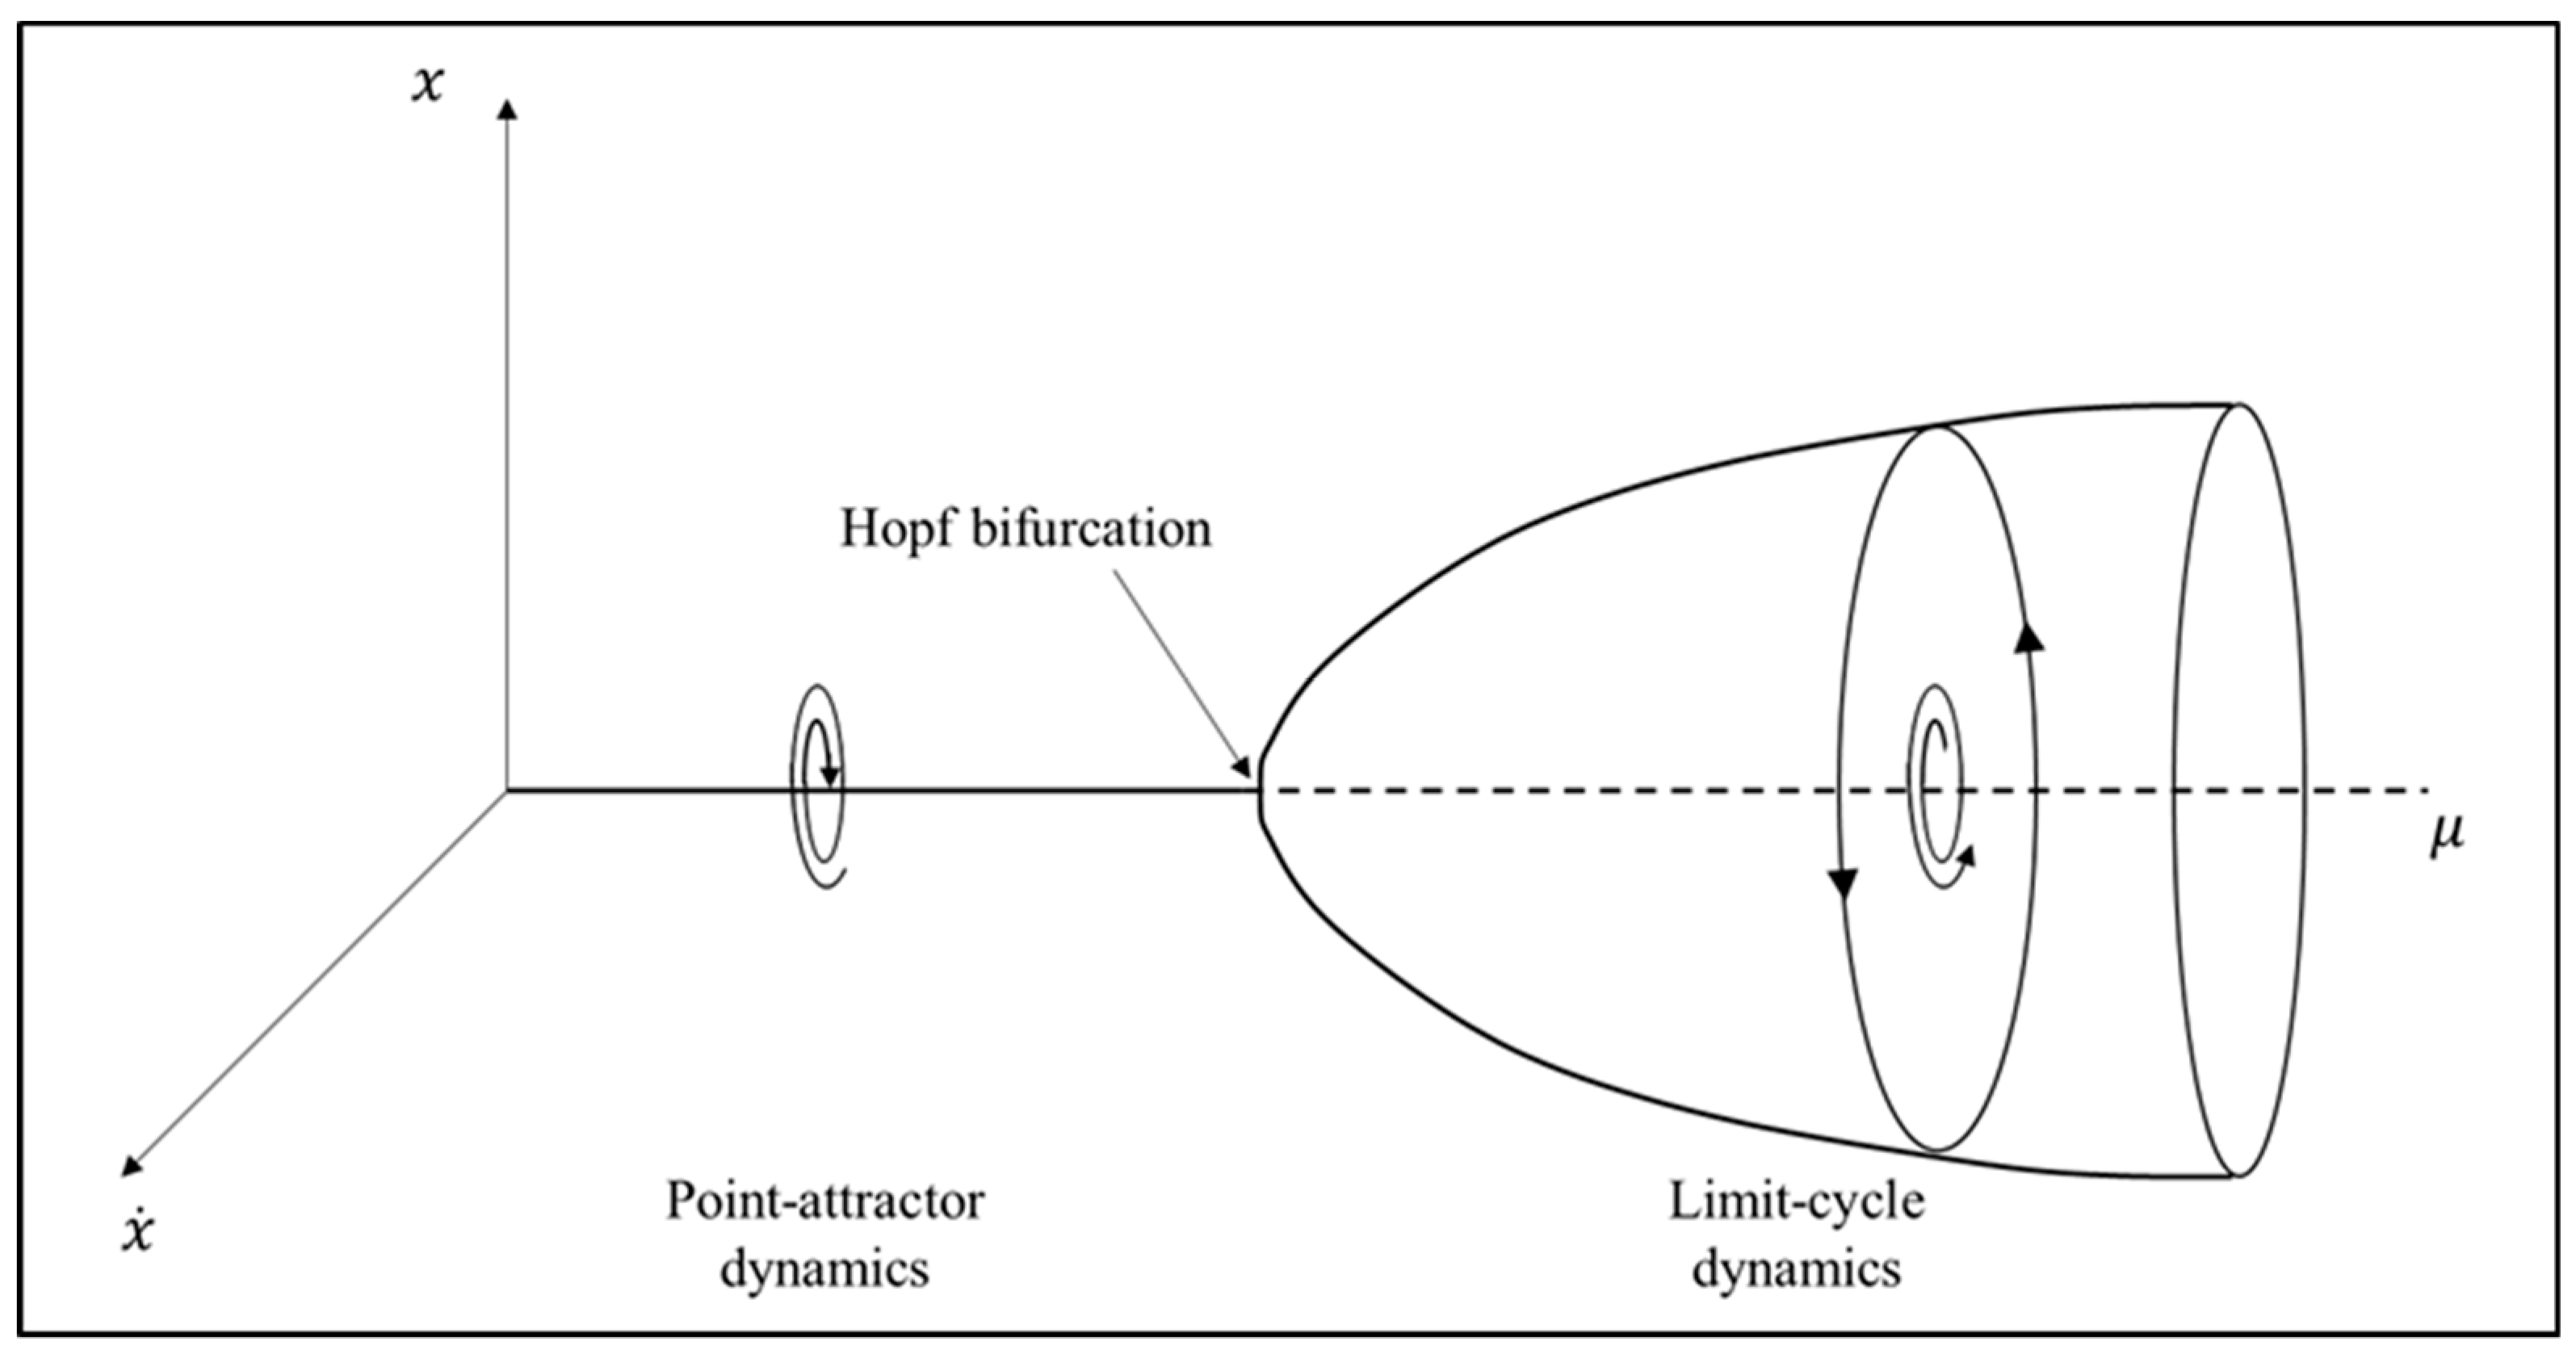
\includegraphics[width=13cm]{math_pics/hopf-bif-pic.png}
	\centering
\end{figure}


\includegraphics[width=11cm]{math_pics/leo.jpg}

\begin{figure}[H]
	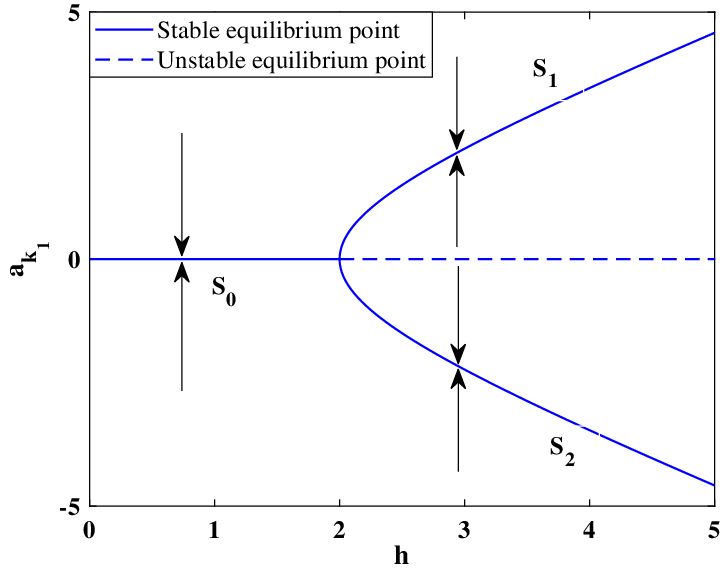
\includegraphics[width=13cm]{math_pics/pitchfork-photo.png}
	\centering
	\caption{Pitchfork bifurcation}
\end{figure}

\hfill\break
//TODO: scrie (si fa mai mult research) despre  \textbf{normal form} si despre cum aproximeaza el sistemul dinamic in jurul punctelor de bifurcatie, ca o sa-ti fie de folos la cam toate punctele de birufcatie sincer pare important si chiarn u stiu de el am vzt in mai multe parti

//TODO: sincer mai bine lasa tbh noone cares as of now
\hfill\break

\subsection{Proving the existence of simple Hopf bifurcations}

Finding necessary conditions for their existence makes use of a tool defined in the previous chapter (\ref{hurwitz_theorem}) the \textbf{Hurwitz matrix}.

Instead, now the characteristic polynomial depends on this new bifurcation parameter $\mu$.

\begin{proposition}\label{symmetric_roots_pair_criterion}
	Take $p_{\mu_0} \in \mathbb{C}^n[Z]$ with $n \geq 2$ and consider $\mu_0$ fixed:
	\[
		p_{\mu_0}(z) = a_0(\mu_0)z^n + a_1(\mu_0)z^{ n-1 } + \dots + a_n (\mu_0)
	\]

	Take $H_i(\mu_0)$ to be $p$'s $i$-th Hurwitz Matrix (\ref{hurwitz_theorem})

	If we have:
	\begin{gather*}
		\text{det }H_1(\mu_0) > 0 , \dots, \text{det }H_{n-2} (\mu_0) > 0. \\
		\Downarrow \\
		p_{\mu_0}(z) \text{ has } \leq 1 \text{ pair of symmetric roots  }
	\end{gather*}

	And $\exists!$ pair of symmetric roots $\iff \text{det}H_{n-1}(\mu_0) = 0$.

	If $a_n(\mu_0) > 0 \implies$ for the pair $\lambda_i, \overline{\lambda_i}$  : Re$(\lambda_i) =$ Re$(\overline{\lambda_i}) = 0$.
\end{proposition}

Now, more specifically, the necessary conditions for a simple Hopf bifurcation are:

\begin{proposition}\label{yangs_criterion}
	(Yang)
	A simple Hopf bifurcation occurs at fixed point $x^*$ and at the parameter threshold $\mu_0$ $\iff$
	\begin{gather*}
		\rom{1} \quad \text{det } H_{ n-1 }(\mu_0) = 0 \text{  and  } a_s(\mu_0) > 0, \\
		\rom{2} \quad 		\text{det }H_1(\mu_0) > 0 , \dots, \text{det }H_{n-2} (\mu_0) > 0 \text{  and  } \\
		\rom{3} \quad \left. \frac{d(\text{det }H_{n-1}(\mu))}{d\mu} \right|_{\mu = \mu_0} \neq 0.
	\end{gather*}
\end{proposition}

\subsection{Ruling out simple Hopf bifurcations}

Directly from criterion \ref{symmetric_roots_pair_criterion} we have a criterion for showing $\nexists \mu$ for which $x(\mu)$ undergoes simple Hopf bifurcations.
\begin{theorem}\label{ruling_out_simple_hopf_bif}

	For the dynamical system $\dot{x} = f_\mu(x)$ assume $\exists$ a curve of steady states $x(\mu)$.
	$p_\mu(z)$ is the characteristic polynomial of degree $s \geq 2$ of the linearization $J(x(\mu), \mu)$, and $H_i(\mu)$ its $i$-th Hurwitz matrix. Given:
	\[
		\text{det }H_1(\mu_0) > 0 , \dots, \text{det }H_{n-2} (\mu_0) > 0. \forall \mu
	\]
	And either:
	\begin{gather*}
		a_s(\mu) \leq 0 \text{whenever  det } H_{s-1} = 0  \\
		\text{or} \\
		\text{det }  H_{s-1}(\mu) \neq 0, \forall \mu    \\
		\Downarrow
	\end{gather*}
	$\nexists$ simple Hopf bifurcation $\forall \mu$ at the steady states $x(\mu)$.
\end{theorem}

\subsection{Convex parameters}\label{convex_paramteres}
With most dynamical systems, if we want to analyze their behavior we have to find, through all possible values if $\exists x^*(\mu)$ fixed points for which bifurcation occur, and hence we need to find any value $\exists \mu$ of the bifurcation parameter for which said bifurcation occurs, throughout our entire domain.

But luck would have it, though that the kind of systems we care about in this thesis, namely chemical reaction systems, defined in more detail in \ref{mass-action_network}, are not like "most" dynamical systems.

They all have a certain structure and their corresponding differential equations look in a way that can be represented more manageably.

Take now a system for a CRN written, written as well in its matrix form, as in \ref{crn_system_matrix_form}
\[
	\dot{x} = f(k,x) :=\Gamma v(k,x)
\]
Where $v$, the flux vector, as in \ref{flux_vector} can be written as:
\[
	v(k, x) = \text{diag}(k)\Psi(x).
\]
as well.
Where diag $: \mathbb{C}^n \rightarrow \mathcal{M}_n(\mathbb{C})$,
\begin{align*}
	(\text{diag}(x))_{i,i} = x_i, \quad \forall i = \overline{1,n} \\
	(\text{diag}(x))_{i,j} = 0, \quad \forall i,j = \overline{1,n} , i \neq j.
\end{align*}
And $\Psi$ is the flux vector, where the reaction rates \ref{reaction_rate} are written without the leading $k_i$'s.

If we want to look into how the system behaves near equilibrium points $x^*$ we have to, just like other systems, study their Jacobian matrix, which, because the flux vector is made of polynomials can be written using this little trick:
\[
	J(k, x)_{\mid x=x^*}=\Gamma \operatorname{diag}\left(v\left(k, x^*\right)\right) \Gamma_L^T \operatorname{diag}\left(\frac{1}{x^*}\right)
\]

Now since $x^*$ is a fixed point, the flux vector satisfies:
\begin{equation}\label{flux_vector_linear_problem}
	\Gamma v(k,x^*) = 0, \quad v \geq 0.
\end{equation}
And so the solutions of (\ref{flux_vector_linear_problem}) are a \textbf{convex polyhedral cone} called the \textbf{flux cone}.

A flux cone is expressed as an $\mathbb{R}_{\geq 0}$ linear combination of it extreme vectors $\left\{ E_1 , \ldots , E_l \right\}$.

\begin{definition}\label{convex_params_definition}
	\textbf{Convex parameters.}
	\begin{equation}\label{flux_cone}
		\boxed{		v=\sum_{i=1}^l \lambda_i E_i=E \lambda, \quad \lambda_i \geq 0, \forall i = \overline{1,l} }
	\end{equation}
	Where $\lambda_i$ are called \textbf{convex parameters}.
\end{definition}
But we also need something to parametrize the $x$'s, so:
\begin{equation}\label{other_convex_parameters}
	\boxed{	h_i=\frac{1}{x_i^*}, \quad i = \overline{1,n} }
\end{equation}
So having this in mind:
\begin{definition}
	A convex parameter vector:
	\[
		(h, \lambda) = (h_1, \ldots, h_n , \lambda_1, \ldots , \lambda_l) \in \mathbb{R}_{>0}^n \times \mathbb{R}_{\geq 0}^{l} : E \lambda \in \mathbb{R}^r_{> 0}.
	\]
	With $E$ the matrix whose columns are the convex polyhedral cone's extreme vectors.
\end{definition}
So we may write the Jacobian using this new coordinate system, which in turn makes its coefficients monomials, instead of the usual polynomial and multiple-term expressions you usually get with these systems, like in Ex. (\ref{bigger_network_example1}).
\newcommand\eqCuzConvex{\stackrel{\mathclap{\normalfont\mbox{\ref{flux_vector_linear_problem}, \ref{convex_params_definition}}}}{=\joinrel=\joinrel=\joinrel=\joinrel=}}

\begin{gather*}
	v(k, x^*) \eqCuzConvex E \lambda	 \\
	\Downarrow \text{ \ref{other_convex_parameters} } \\
	\boxed{J(k,x)_{|x=x^{*}}=J(h,\lambda)=\Gamma \text{diag}(E\lambda)\Gamma_{L}^{T}\text{diag}(h)}
\end{gather*}

We could, of course turn this convex vector back into the regular coordinate system:

Given:
\begin{gather*}
	(h,\lambda) \Downarrow \\
	\text{Let  } x^* \in \mathbb{R}^n , \boxed{
		x^*_i = \frac{1}{h_i} , i = \overline{1,n}
	} \\
	\boxed{
		k = \text{diag}(\Psi(h)) E \lambda \in \mathbb{R}^r_{> 0}
 }
\end{gather*}

\hfill\break
//TODO: Aici trebuie re-introducere la notatia specifica pt reactiile chimice, si adica mai bine te pui sa vb despre asta in primele capitole de "Introduction to chemical reaction networks"
si asta o sa fie pt orice fel de reactii chimice, nu doar pt astea de mai jos:
Poti sa te folosesti nu numa de prezentare da si din lucrarea lui conradi ca zice chestii mai specifice asa sa zic nuj.
//TODO sa mai zici si tu cand e si cand te intereseaza ce e ala flux cone si cum functioneste
\hfill\break

\section{What is a Phosphorylation-Dephosphorylation CRN?}

\hfill\break
//TODO: Povestesti frumos specific pt asta ce sunt, din nou, te iei din ce s-a vb in prezentare da poate un pic si din ala alu conradi
\hfill\break

Phosphorylation of proteins occurs in cycles, which are fueled by $3$ proteins which are the ingredients: A substrate $S$ and $2$ enzymes: kinase ($K$) and phosphatase ($F$).

The one that starts this chain is the kinase ($K$), attaching phosphate groups onto the substrate, phosphorylating it.

Then, phosphatase ($F$) comes in and undoes all the hard work kinase ($K$) put in and removes the phosphate groups, now dephosphorylating the substrate.

\hfill\break
These cycles are a particular case of a broader type of what are called \textbf{posttranslational modification (PTM) systems.} Another example would be, for instance \textbf{methylation}.

The reason we care about them is their key implication in \textbf{ signal transduction}, which is the process our cells use to communicate with one-another. Any disturbance in this system is linked to its own class of health complications in our body.

Basically, do these biochemical systems induce periodic solutions as in (\ref{hopf_bif_def}), likening clocks, or do they have multiple steady-states (\textbf{capacity for bistability}), likening switches?

What these all have in common, though are the \textbf{building blocks} used to create them:
\begin{equation}\label{ptm_building_blocks}
	S+M \xleftrightharpoons[k_1]{k_2} SM \xrightarrow{k_3} S^* + M \quad \mathrm{~and~} \quad S^* + U \xleftrightharpoons[k_4]{k_5} S^* U \xrightarrow{k_6} S + U
\end{equation}

What's familiar to the previous example is the presence of a substrate ($S$), which forms the \textbf{complex} ($SM$) with the \textbf{modifier} ($M$), which - as the name implies - modifies ($S$) to become ($S^*$), which then dissociates with ($M$);

And just like in dephosphorylation, another modifier ($U$) can come in and undo the entire hustle ($M$) did.

So the \textbf{phosphorylation version of this would be}:
\begin{gather*}\label{phosphorylation_reaction_basis}
	S_0 + K \xleftrightharpoons[k_1]{k_2} K S_0 \xrightarrow{k_3} S_1 + K  \xleftrightharpoons[k_4]{k_5} \ldots K S_{n-1} \xrightarrow{k_{ 3n}} S_n + K  \\
	\text{ for the phosphorylation side, and} \\
	S_n + F \xleftrightharpoons[k_{2(n+1)}]{k_{2n+1}} F S_n \xrightarrow{k_{2n + 3}} S_{n-1} + F  \xleftrightharpoons[k_{2n + 4}]{k_{2n + 5}} \ldots F S_{1} \xrightarrow{k_{6n}} S_0 + F  \\
	\text{ for the dephosphorylation side, and}
\end{gather*}
Which phosphorylates the substrate ($S$) up to a certain number of phosphate groups $n$, and then \textbf{de}phosphorylates it back to 0, where the subscript notation $S_i ;  i = \overline{1,n}$ represents the substrate ($S$) with its $i$ phosphate groups.

The system above represents a \textbf{distributive} cycle, meaning each bounding site of ($K$) and ($F$) (de)phosphorylate only one single phosphate group.

As opposed to a \textbf{processive} one, which would look something like:
\begin{equation*}
	S_0 + K \xrightleftharpoons[k_2]{k_1} S_0 K \xrightarrow{k_3} S_1 K \xrightarrow{k_4} S_2 + K
\end{equation*}
For a binding one, and
\begin{equation*}
	S_2 + F \xrightleftharpoons[k_2]{k_1} S_2 F \xrightarrow{k_3} S_1 F \xrightarrow{k_4} S_0 + F
\end{equation*}
For the unbinding operation.

//TODO: de ce ne intereseaza specfici phospho, de phosho?

\subsection{Cyclic and mixed distributive and processive Phosphorylation-Dephosphorylation CRN}


\chapter{CoNtRoL Simulations Web Application}
\label{ch:web-app}

\textit{ Here we will present the open-source Web application developed for easing work involving chemical reaction networks, hopefully for students and researchers one day. It can be used for obtaining numerical analysis of chemical reaction networks, as well as plotting species against time, one another and even the graph of a network. We'll present the technologies used throughout the project, how to run it locally and a couple of usage examples involving what we've presented in the previous chapters. A lot of the heavy lifting was done by these libraries \footcite{10.1093/bioinformatics/btac730, xu2023SbmlDiagrams, medley2018tellurium, choi2018Tellurium}. I've also had the opportunity of contributing a commit or two to \href{https://github.com/sys-bio/tellurium}{Tellurium}, one of core libraries, during the making of this app.}

\subsection{Overview of the technologies}
The website is a back-end application built in \textbf{Python}, a programming language known for its use in basically every single science, including natural sciences so it's a no-brainer when in comes to plotting.

The web server is built using \textbf{Flask}, a lightweight web app framework and the webpages served are server-side rendered by Flask's template engine depedency - \textbf{Jinja}.
\\
The crux of the functionality is aided by the Python library \textbf{Tellurium}\footcite{choi2018Tellurium,medley2018tellurium}; which is, as their docs say; "A Python Environment for Reproducible Dynamical Modeling of Biological Networks". It uses a subset of the Systems Biology Markup Language ( \textbf{SBML})\footcite{xu2023SbmlDiagrams,bornstein2008Libsbml, 10.1093/bioinformatics/btac730} called \textbf{Antimony} which can be used in this app to create a Chemical Reaction Network, as well as the friendlier selects form. So the bits doing the magic are the calls to \verb|road_runner.loada()| which are used to \textbf{\textit{load}}    \textbf{a}ntimony code into the model.
the \verb|road_runner.simulate()| function is then used for running and obtaining sumulation data, followed by \verb|road_runner.plot()|, which in turn calls a \verb|matplotlib| headless backend for writing the plotted results to a file.

\subsection{Running it}
As explained in the \verb|README| of \href{https://github.com/viktorashi/Open-CoNtRol}{the project}, installing and running locally is a bit more tedious and highly depends on which opperating system you're running, but the general overview goes, kind-of like this:. \\\\

\tikz\draw[black,fill=black] (0,0) circle (.5ex); clone the project

\begin{lstlisting}[language=bash]
    git clone https://github.com/viktorashi/Open-CoNtRol.git
\end{lstlisting}

\tikz\draw[black,fill=black] (0,0) circle (.5ex); \textbf{c}hange \textbf{d}irectory into it.

\begin{lstlisting}[language=bash]
    cd Open-CoNtRol
\end{lstlisting}

\tikz\draw[black,fill=black] (0,0) circle (.5ex); (optionally) install \href{https://virtualenvwrapper.readthedocs.io/en/latest/}{virtualenvwrapper} (which I reccomend) and create a \textbf{virtual environment}

\begin{lstlisting}[language=bash]
    mkvirtualenv control #or whatever you want to name it
\end{lstlisting}

Now here comes the part depending on your OS: You need to install \href{https://pygraphviz.github.io}{PyGraphviz}, which is essential to plotting the Graph view of networks, but it uses a C/C++ back-end so it's not as easy a simple \verb|pip install|

\tikz\draw[black,fill=black] (0,0) circle (.5ex); On Linux:
\begin{lstlisting}[language=bash]
    sudo apt-get install graphviz graphviz-dev
    pip install pygraphviz
\end{lstlisting}

\tikz\draw[black,fill=black] (0,0) circle (.5ex); On macOS:
\begin{lstlisting}[language=bash]
    #first install \href{https://brew.sh}{Homebrew}
    /bin/bash -c "$(curl -fsSL https://raw.githubusercontent.com/Homebrew/install/HEAD/install.sh)"
    brew install graphviz
    pip install pygraphviz
\end{lstlisting}

\tikz\draw[black,fill=black] (0,0) circle (.5ex); And if that doesn't work (usually because of newer macOS versions), change the third part of the installation like so:

\begin{lstlisting}[language=bash]
pip install --config-settings="--global-option=build_ext" \
            --config-settings="--global-option=-I$(brew --prefix graphviz)/include/" \
            --config-settings="--global-option=-L$(brew --prefix graphviz)/lib/" \
            pygraphviz
\end{lstlisting}

\tikz\draw[black,fill=black] (0,0) circle (.5ex); For Windows, I just use \href{https://learn.microsoft.com/en-us/windows/wsl/install}{WSL}:

Now this part is the same no matter which OS you use

\tikz\draw[black,fill=black] (0,0) circle (.5ex); install the rest of the requirements

\begin{lstlisting}[language=bash]
    pip install -r requirements.txt
\end{lstlisting}

\tikz\draw[black,fill=black] (0,0) circle (.5ex); Now I suggest you just
\begin{lstlisting}[language=bash]
    flask run
\end{lstlisting}

\tikz\draw[black,fill=black] (0,0) circle (.5ex); Orrr
\begin{lstlisting}[language=bash]
    python -m flask run
\end{lstlisting}

\tikz\draw[black,fill=black] (0,0) circle (.5ex);
But if that doesn't work, give the \verb|run_script.sh| execute permissions

\begin{lstlisting}[language=bash]
    chmod +x ./run_script.sh
\end{lstlisting}

\tikz\draw[black,fill=black] (0,0) circle (.5ex);
and give it a shot

\begin{lstlisting}[language=bash]
    ./run_script.sh
\end{lstlisting}

Among the wall of output will also be the line showing the address your server is located at, for example:
\verb|* Running on http://127.0.0.1:5000|, address at which you'll be greeted with this screen

\[
	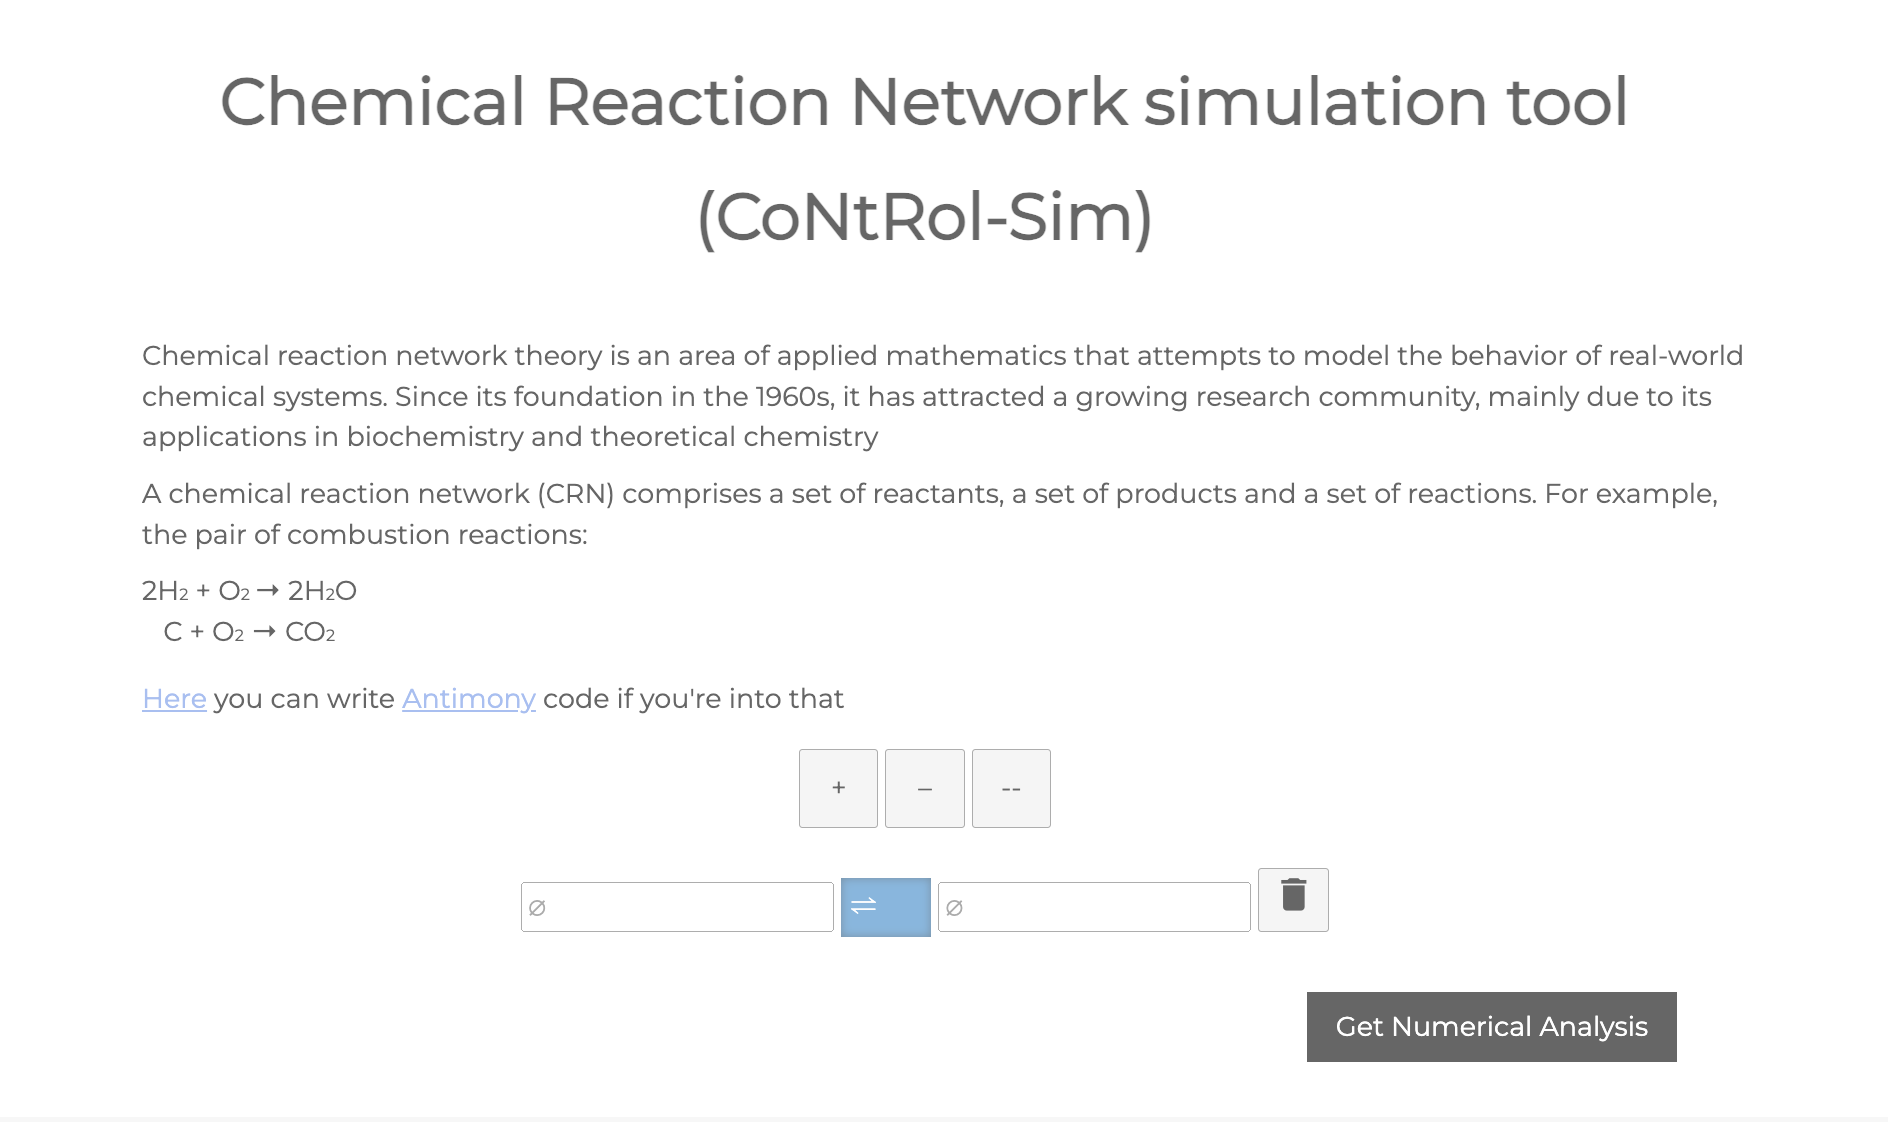
\includegraphics[width=13cm]{app_photos/control_home_screen.png}\\
\]

You can either use this as a starting point or the page located at the \verb|/antimony| path:

\[
	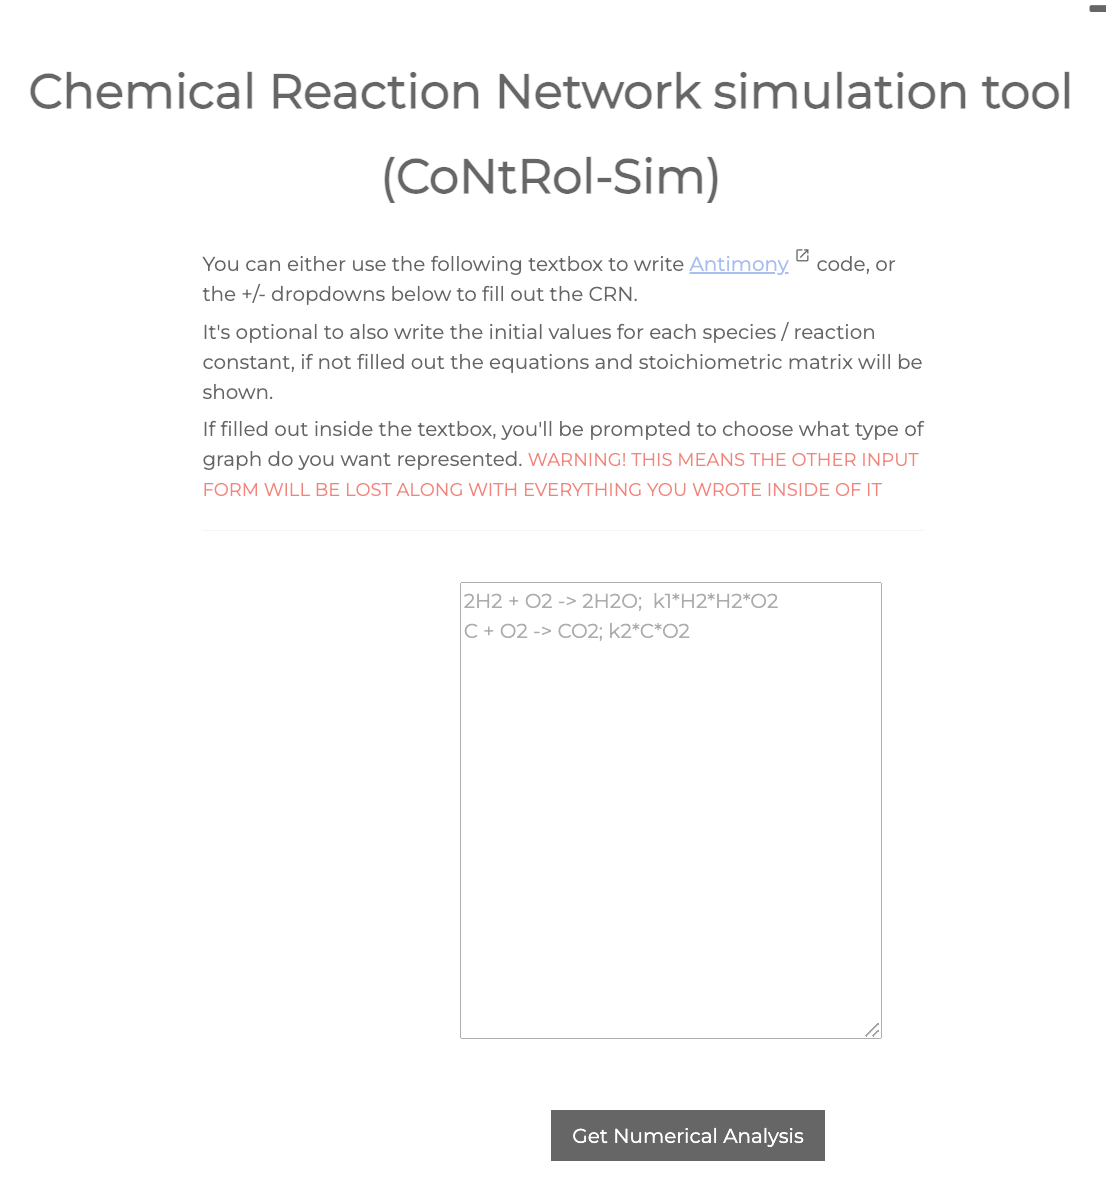
\includegraphics[width=13cm]{app_photos/control_antimony_home.png}\\
\]
Both of these redirect to \verb|/numerical_analysis| analysing the system \ldots well, numerically.
As an example, this Antimony code:

\begin{lstlisting}
S0 -> KS1; k1*S0
KS1 -> S2; k2*KS1
S2 + F -> FS2; k3*S2*F
FS2 -> F; k4*FS2
F -> S0 + F; k5*F
\end{lstlisting}

and its longer to write alternative:

\[
	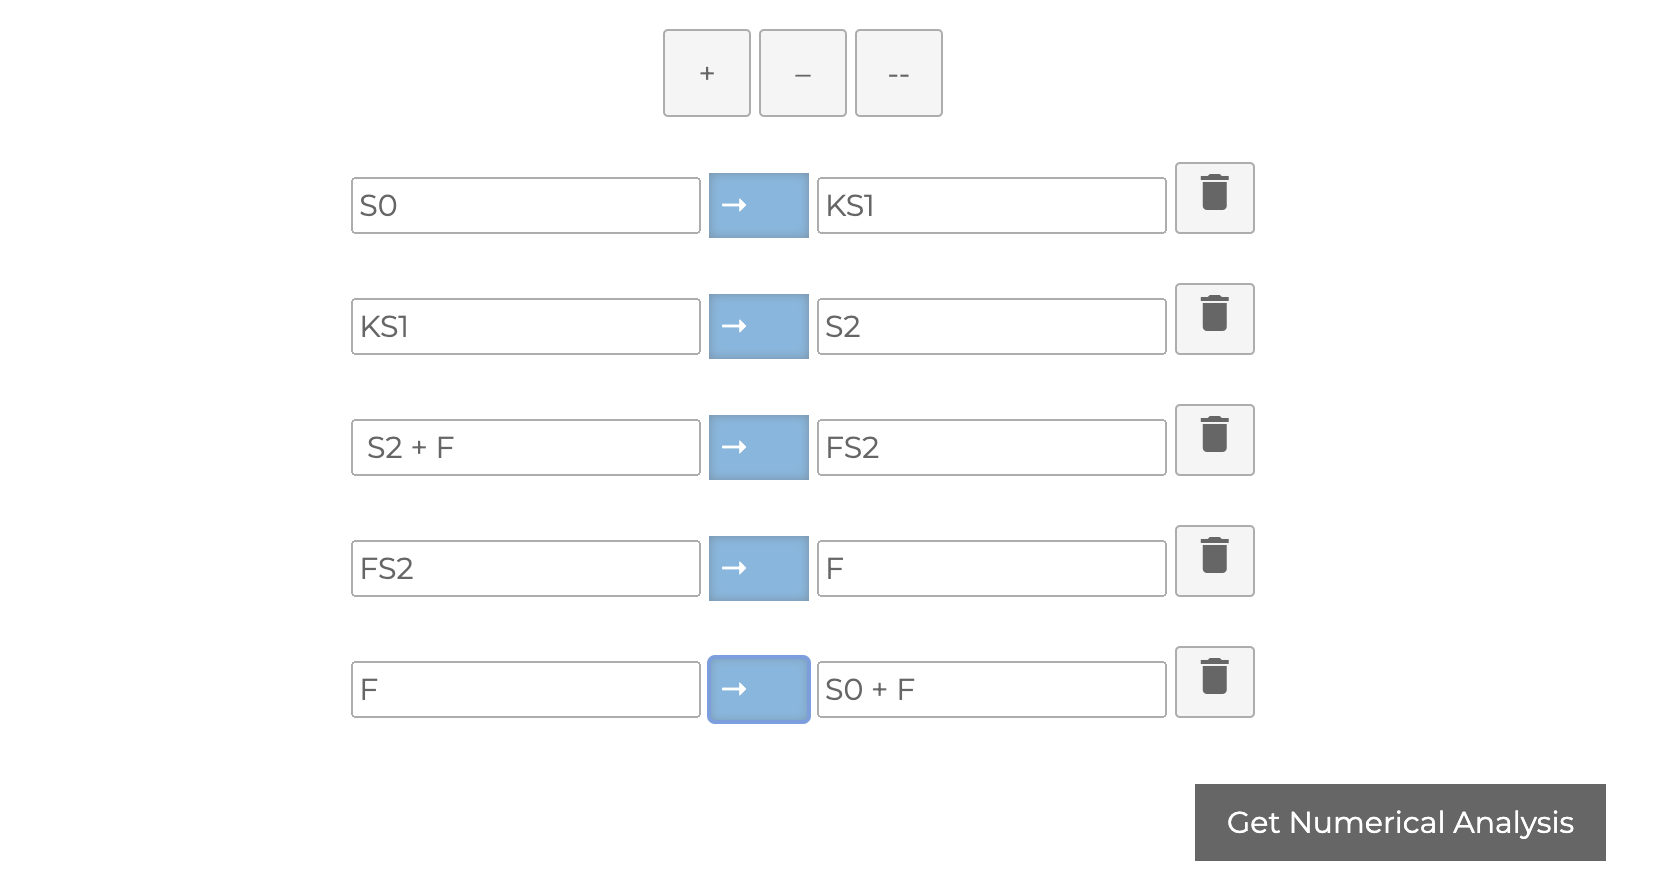
\includegraphics[width=13cm]{app_photos/creca-prima-data-cand-am-scris-asta.png}\\
\]

both yield the same numerical analysis results:

\[
	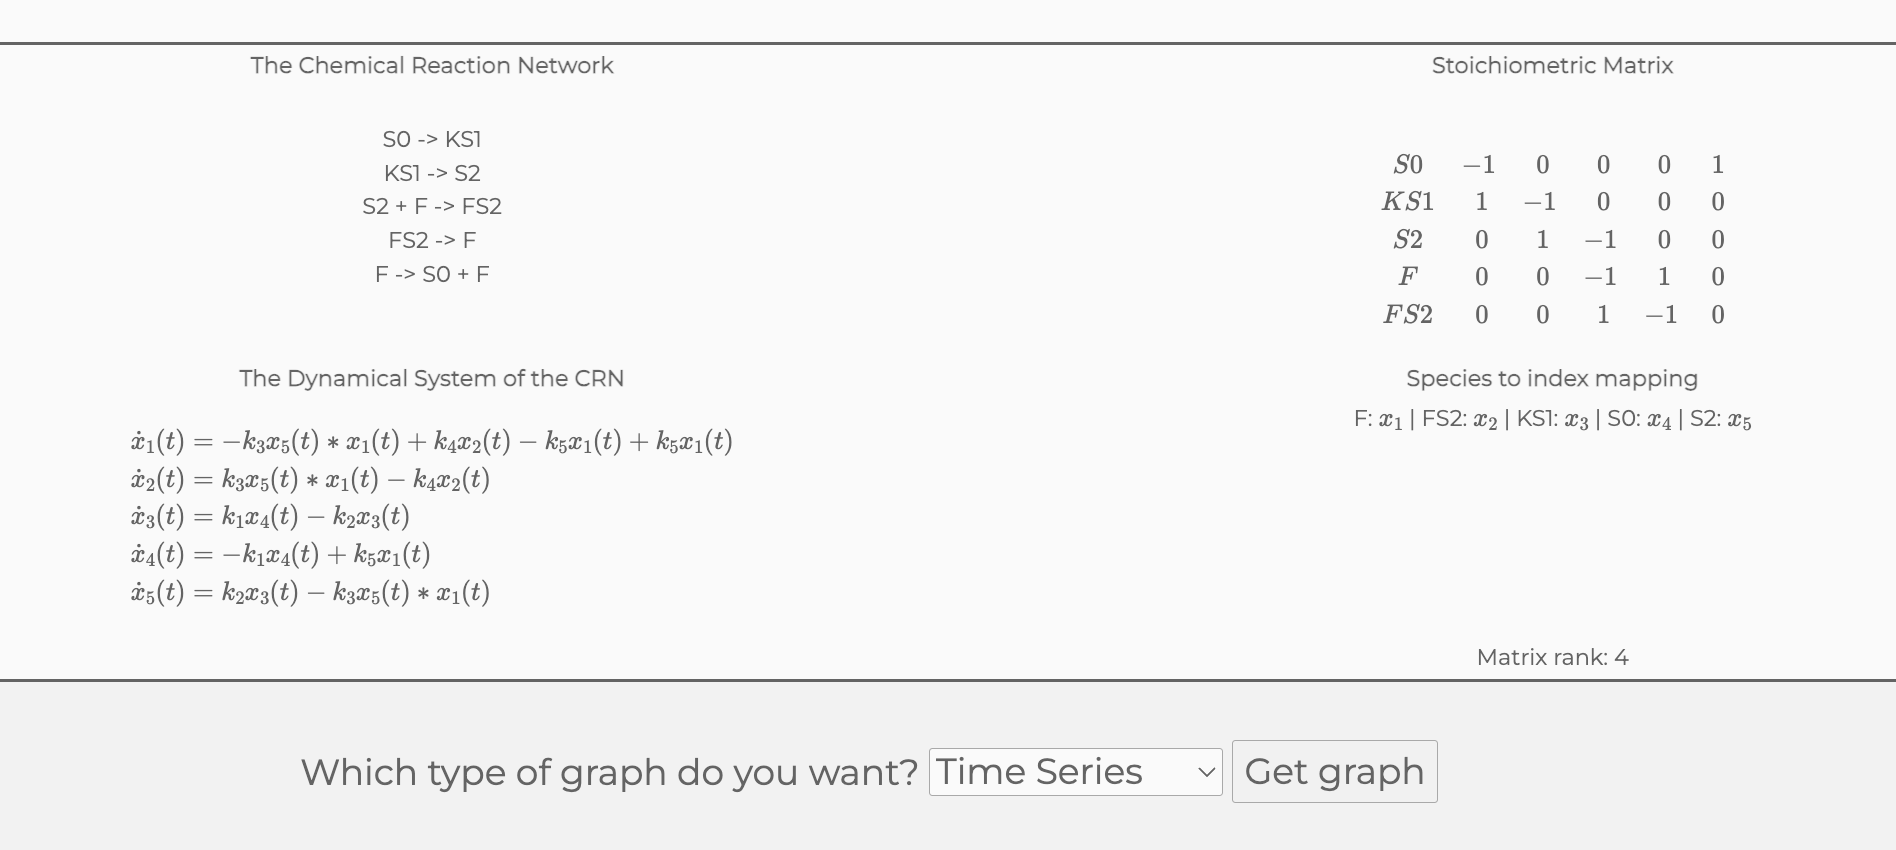
\includegraphics[width=13cm]{app_photos/numerical_analysis.png}\\
\]

from here, one can choose from a selection of graphs they can represent given this system, the default one being the time series representation:

\[
	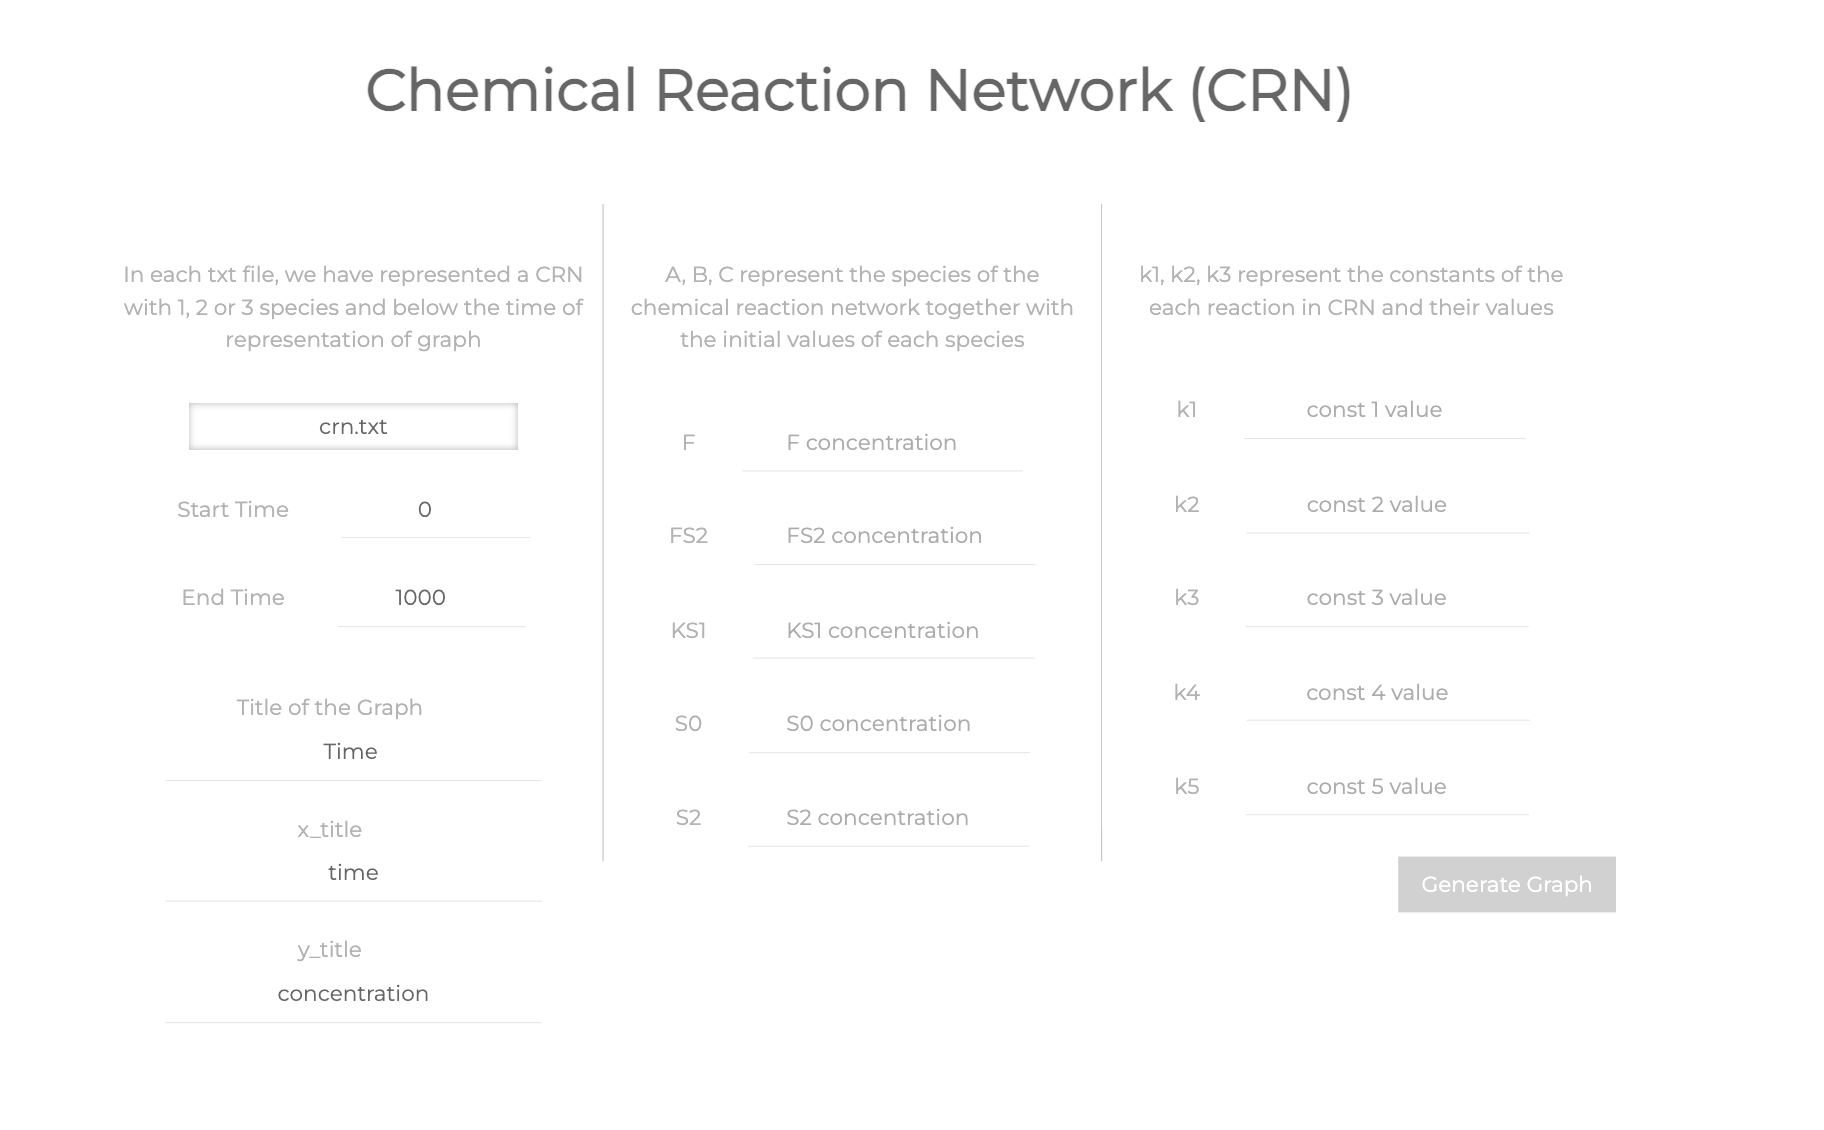
\includegraphics[width=13cm]{app_photos/tsr-input.png}\\
\]

from which we fill out the initial values of the concentrations for each species as, well as the reaction rates. So given, for example the values:\label{last_system_init_cond}
\begin{lstlisting}
    F = 0.874108
    FS2 = 7.620157734
    KS1 = 7.620157734
    S0 = 7.270157734
    S2 = 0.6000000000

    k1 = 0.1329759342
    k2 = 0.1329759342
    k3 = 2
    k4 = 0.1329759342
    k5 = 1
\end{lstlisting}

outcomes the graph:

\[
	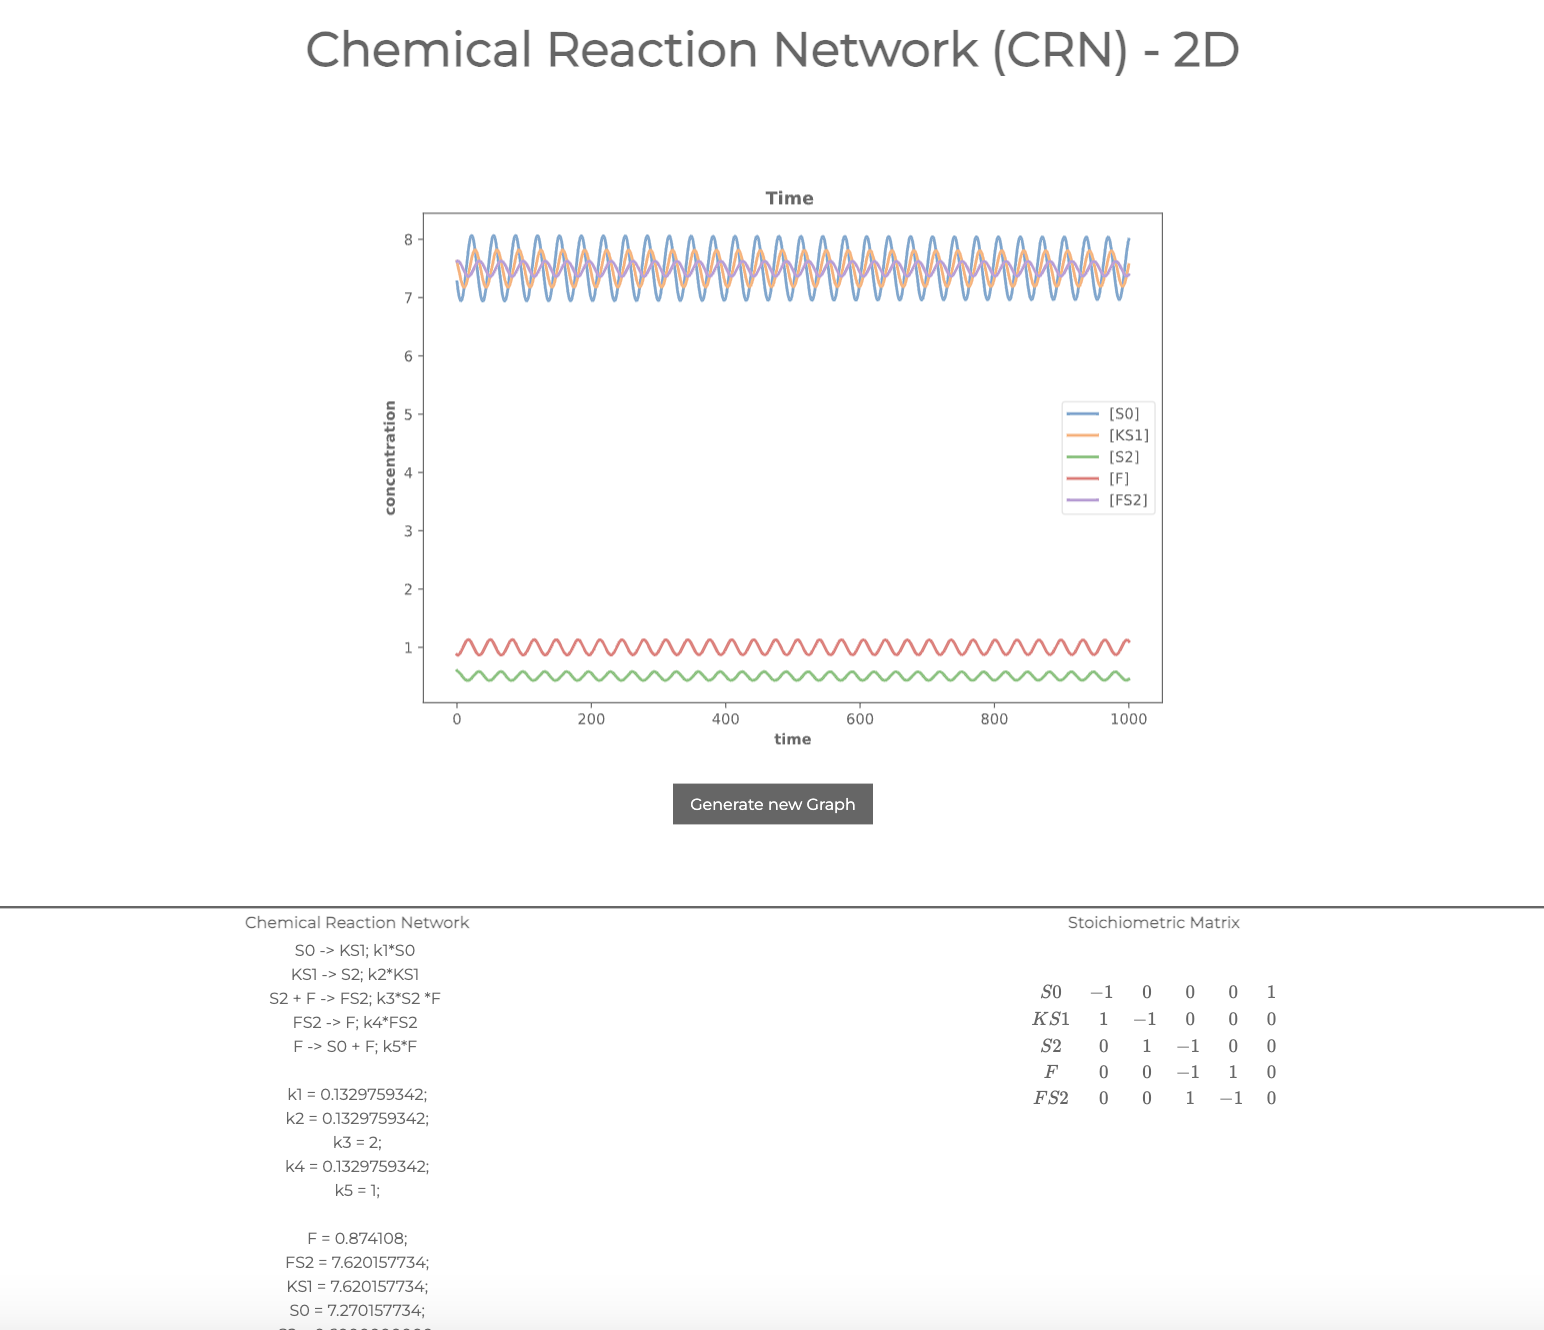
\includegraphics[width=13cm]{app_photos/a-graph-indeed.png}\\
\].

\subsection{The bottom line}

So this is how the workflow of the app typically goes. \\
$
\begin{WithArrows} & \textit{write out your system} \rightarrow \textit{get numerical analysis} \rightarrow \textit{choose your desired graph} \Arrow{\textit{fill out data values}}  \\
	& \hfill \textbf{Voilà}
\end{WithArrows}
$

%\addcontentsline{toc}{chapter}{Concluzii}
%\addcontentsline{toc}{chapter}{Conclusions}

\printbibliography

\end{document}
